% PSV Guard white paper.
% Build: make -C docs/whitepaper   (figures: go run -tags whitepaper ./docs/whitepaper/figdata)
\documentclass[11pt,a4paper]{article}

\usepackage[T1]{fontenc}
\usepackage[utf8]{inputenc}
\usepackage{libertinus}
\usepackage{libertinust1math}
\usepackage{float}
\usepackage[scaled=0.86]{beramono}
\usepackage[a4paper,margin=2.5cm,headheight=14pt]{geometry}
\usepackage{microtype}
\usepackage{amsmath,amssymb}
\usepackage{graphicx}
\usepackage{booktabs,tabularx,multirow}
\usepackage[table]{xcolor}
\usepackage{tikz}
\usepackage{pgfplots,pgfplotstable}
\usepackage{caption,subcaption}
\usepackage{enumitem}
\usepackage{fancyhdr}
\usepackage{titlesec}
\usepackage[hidelinks]{hyperref}
\usepackage[capitalise,noabbrev]{cleveref}
\usepackage{siunitx}
\usepackage{tcolorbox}

\pgfplotsset{compat=1.18}
\usetikzlibrary{arrows.meta,positioning,calc,shapes.geometric,fit,backgrounds,decorations.pathreplacing,patterns}
\usepgfplotslibrary{fillbetween}

\graphicspath{{figures/}{figures/generated/}{../images/}}

% Generated by docs/whitepaper/figdata. Do not edit.
\newcommand{\LocalFPS}{60.00}
\newcommand{\LocalSource}{1280$\times$720}
\newcommand{\LocalAnalysed}{640$\times$360}
\newcommand{\LocalFirstActivity}{1.02}
\newcommand{\LocalFirstFlashing}{1.60}
\newcommand{\LocalFirstFail}{1.60}
\newcommand{\LocalFirstCover}{1.30}
\newcommand{\LocalDecidedFails}{24}
\newcommand{\LocalMisses}{0}
\newcommand{\LocalCoverSeconds}{4.72}
\newcommand{\LocalSeconds}{4.00}
\newcommand{\ColorsFPS}{29.97}
\newcommand{\ColorsSource}{1920$\times$1080}
\newcommand{\ColorsAnalysed}{640$\times$360}
\newcommand{\ColorsFirstActivity}{0.03}
\newcommand{\ColorsFirstFlashing}{0.33}
\newcommand{\ColorsFirstFail}{0.33}
\newcommand{\ColorsFirstCover}{0.18}
\newcommand{\ColorsDecidedFails}{230}
\newcommand{\ColorsMisses}{0}
\newcommand{\ColorsCoverSeconds}{9.83}
\newcommand{\ColorsSeconds}{8.01}
\newcommand{\FlashFPS}{60.00}
\newcommand{\FlashSource}{1280$\times$720}
\newcommand{\FlashAnalysed}{640$\times$360}
\newcommand{\FlashFirstActivity}{1.00}
\newcommand{\FlashFirstFlashing}{1.60}
\newcommand{\FlashFirstFail}{1.60}
\newcommand{\FlashFirstCover}{1.30}
\newcommand{\FlashDecidedFails}{24}
\newcommand{\FlashMisses}{0}
\newcommand{\FlashCoverSeconds}{4.72}
\newcommand{\FlashSeconds}{4.00}
\newcommand{\ScrollFPS}{60.00}
\newcommand{\ScrollSource}{1280$\times$720}
\newcommand{\ScrollAnalysed}{640$\times$360}
\newcommand{\ScrollFirstActivity}{0.02}
\newcommand{\ScrollFirstFlashing}{0.12}
\newcommand{\ScrollFirstFail}{-1.00}
\newcommand{\ScrollFirstCover}{-1.00}
\newcommand{\ScrollDecidedFails}{0}
\newcommand{\ScrollMisses}{0}
\newcommand{\ScrollCoverSeconds}{0.00}
\newcommand{\ScrollSeconds}{4.00}
\newcommand{\AdFPS}{23.98}
\newcommand{\AdSource}{1920$\times$1080}
\newcommand{\AdAnalysed}{640$\times$360}
\newcommand{\AdFirstActivity}{0.54}
\newcommand{\AdFirstFlashing}{0.83}
\newcommand{\AdFirstFail}{-1.00}
\newcommand{\AdFirstCover}{-1.00}
\newcommand{\AdDecidedFails}{0}
\newcommand{\AdMisses}{0}
\newcommand{\AdCoverSeconds}{0.00}
\newcommand{\AdSeconds}{5.00}
\newcommand{\SnapFlasha}{1.100}
\newcommand{\SnapFlashb}{1.300}
\newcommand{\SnapFlashc}{1.600}
\newcommand{\SnapLocala}{1.100}
\newcommand{\SnapLocalb}{1.300}
\newcommand{\SnapLocalc}{1.600}
\newcommand{\SnapScrolla}{0.033}
\newcommand{\SnapScrollb}{0.067}
\newcommand{\SnapScrollc}{0.117}


% Palette, matched to the heatmaps the figure generator draws.
\definecolor{brand}{HTML}{E11D48}
\definecolor{brandDark}{HTML}{BE123C}
\definecolor{ink}{HTML}{1F2329}
\definecolor{muted}{HTML}{5B6270}
\definecolor{cold}{HTML}{3884FF}
\definecolor{hot}{HTML}{FFB020}
\definecolor{flash}{HTML}{E6283C}
\definecolor{calm}{HTML}{2E9E6A}
\definecolor{panel}{HTML}{F4F5F7}

\hypersetup{pdftitle={Covering Flashing Before It Fails},pdfauthor={Brian Nunez},
  pdfsubject={Photosensitive epilepsy and real-time flash detection in PSV Guard}}

\titleformat{\section}{\Large\bfseries\color{ink}}{\color{brand}\thesection}{0.8em}{}
\titleformat{\subsection}{\large\bfseries\color{ink}}{\color{brand}\thesubsection}{0.8em}{}
\titleformat{\subsubsection}{\normalsize\bfseries\color{ink}}{\thesubsubsection}{0.8em}{}

\pagestyle{fancy}
\fancyhf{}
\fancyhead[L]{\small\color{muted}Covering Flashing Before It Fails}
\fancyhead[R]{\small\color{muted}Brian Nunez}
\fancyfoot[C]{\small\thepage}
\renewcommand{\headrulewidth}{0.4pt}

\captionsetup{font=small,labelfont={bf,color=ink},margin=0.5cm}
\setlist{itemsep=2pt,topsep=4pt}
\sisetup{group-minimum-digits=4}

\newcommand{\psv}{\textsf{psv}}
\newcommand{\guard}{PSV Guard}
\newcommand{\code}[1]{\texttt{#1}}

% A boxed note.
\newtcolorbox{keypoint}[1]{colback=panel,colframe=brand!70,boxrule=0.6pt,arc=3pt,left=8pt,right=8pt,top=6pt,bottom=6pt,
  fontupper=\normalsize,before upper={\textbf{\color{brandDark}#1.}\ }}

\begin{document}

% ---------------------------------------------------------------- Cover
\begin{titlepage}
  \thispagestyle{empty}
  \begin{tikzpicture}[remember picture,overlay]
    \fill[brand] (current page.north west) rectangle ([yshift=-0.9cm]current page.north east);
    \fill[ink] (current page.south west) rectangle ([yshift=0.5cm]current page.south east);
  \end{tikzpicture}
  \vspace*{3.2cm}
  \begin{center}
    
\includegraphics[width=3.2cm]{icon.png}\\[1.6cm]
    {\fontsize{30}{36}\selectfont\bfseries\color{ink} Covering Flashing\\[4pt] Before It Fails\par}
    \vspace{0.9cm}
    {\Large\color{muted} Photosensitive epilepsy, pixel-level flash detection,\\[2pt]
      and real-time protection in PSV Guard\par}
    \vspace{0.6cm}
    {\color{brand}\rule{4cm}{1.2pt}}
    \vspace{2.4cm}

    {\Large\bfseries Brian Nunez\par}
    \vspace{0.3cm}
    {\large\color{muted} White paper \textperiodcentered{} November 2026\par}
  \end{center}
  \vfill
  \begin{center}
    \small\color{muted}
    PSV Guard is an experimental aid. It reduces exposure to flashing content but does not eliminate it,\\
    and it does not detect spatial patterns. Nothing in this paper is medical advice.
  \end{center}
\end{titlepage}

% ---------------------------------------------------------------- Abstract
\setcounter{page}{2}
\section*{Abstract}

Flashing light can trigger seizures in people with photosensitive epilepsy. For decades, broadcasters and accessibility standards have defined when flashing becomes hazardous. A sequence is hazardous when it is bright enough, covers enough of the field of view, and alternates often enough within one second. These rules are applied before content is published, by checking a finished video. Content shown on a computer is rarely checked: web pages, games, video calls, and other people's screens reach the viewer unchecked.

This paper describes two pieces of software that apply those rules to pixels as they reach the screen. The first, \psv{}, is a flash detector. It reduces the guidelines to per-pixel rules: luminance and saturated-red transitions, merged ramps, alternation, and a one-second count. It then finds the regions in which enough of those pixels transition together. It is exact with respect to its stated rules, and it can watch a live stream, reporting in every frame how far each pixel is from flashing. The second, \guard{}, is a macOS menu bar app. It captures every display at 60 frames per second, streams each one through \psv{}, and covers the parts of the screen where flashing is building up, before \psv{} would decide that the content fails.

Using \psv{}'s own example videos and synthetic clips, we show that a pixel-level count alone cannot separate flashing from scrolling text. A measure we call \emph{fill} can: the share of each transitioning cell that changes together. On the clips measured here, \guard{} covers failing content 0.15--0.30\,s before its first failing frame, with no frame of a decided failure left uncovered. Scrolling text and a passing advertisement stay uncovered. We also report the limits we measured: small flashing, unrelated motion that starts while a cover is up, and the system's own animations.

\vspace{0.4cm}
\tableofcontents
\clearpage

% ---------------------------------------------------------------- 1
\section{Introduction}

On 16 December 1997, an episode of the \emph{Pocket Monsters} cartoon was broadcast in Japan. It contained a few seconds of red and blue light alternating about twelve times a second. Around seven hundred people, most of them children, were taken to hospital that evening with seizure symptoms~\cite{takahashi1998}. The episode was never shown again, and broadcasters in many countries tightened their checks on flashing images. Today, broadcast guidance~\cite{itu1702,ofcom}, an ISO ergonomics standard~\cite{iso9241391} and the Web Content Accessibility Guidelines~\cite{wcag22} all describe the same kind of hazard in similar terms.

Those rules are applied to content before it is published, by running a checked file through an analyser. The screen of a personal computer is different. It shows content that nobody checked: advertisements, games, short videos, animated web pages, screen shares and notifications. These are composed together at the moment they are displayed. A viewer who is photosensitive has no way to know in advance that the next second of their screen will be safe.

\guard{} takes the opposite approach. Instead of checking content, it watches what the screen actually shows and covers the flashing as it begins. \Cref{fig:overview} shows the idea. Each display is captured, every frame is measured by the \psv{} flash detector, and a covering policy decides, frame by frame, which parts of the screen to dim.

\begin{figure}[ht]
  \centering
  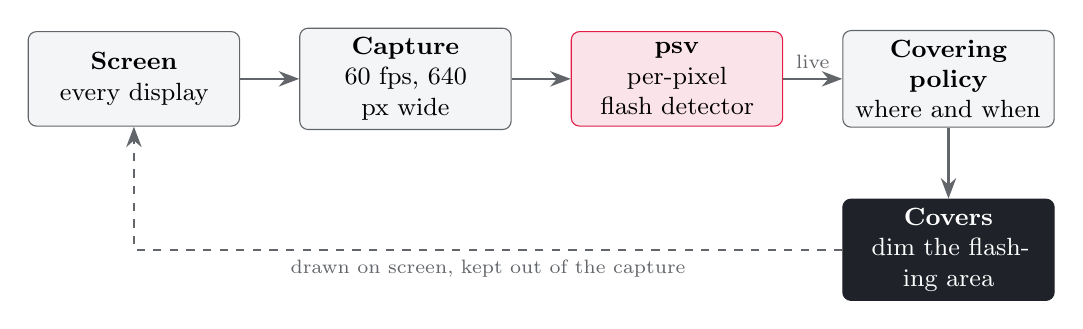
\begin{tikzpicture}[
      box/.style={draw=ink!70,rounded corners=3pt,fill=panel,minimum height=1.2cm,text width=2.45cm,align=center,font=\small},
      arr/.style={-{Stealth[length=2.6mm]},thick,ink!70}]
    \node[box] (screen) {\textbf{Screen}\\every display};
    \node[box,right=0.75cm of screen] (cap) {\textbf{Capture}\\60 fps, 640 px wide};
    \node[box,right=0.75cm of cap,fill=brand!12,draw=brand] (psv) {\textbf{psv}\\per-pixel flash detector};
    \node[box,right=0.75cm of psv] (pol) {\textbf{Covering policy}\\where and when};
    \node[box,below=0.9cm of pol,fill=ink,text=white,draw=ink] (cover) {\textbf{Covers}\\dim the flashing area};
    \draw[arr] (screen) -- (cap);
    \draw[arr] (cap) -- (psv);
    \draw[arr] (psv) -- node[above,font=\scriptsize]{live} (pol);
    \draw[arr] (pol) -- (cover);
    \draw[arr,dashed] (cover.west) -| node[pos=0.25,below,font=\scriptsize,align=center]{drawn on screen, kept out of the capture} (screen.south);
  \end{tikzpicture}
  \caption{\guard{} at a glance. Covers are drawn over the screen but excluded from the capture, so they never feed back into the analysis.}
  \label{fig:overview}
\end{figure}

This paper explains the whole chain. \Cref{sec:pse} summarises what is known about photosensitive epilepsy and how the guidelines turn it into measurable thresholds. \Cref{sec:psv} describes how \psv{} applies those thresholds to pixels, both for a finished video and for a live stream. \Cref{sec:guard} describes how \guard{} turns \psv{}'s live measurement into covers, and why the obvious rule fails. \Cref{sec:results} reports measured results, \cref{sec:limits} the limits, and \cref{sec:conclusion} concludes.

\begin{keypoint}{Scope}
\guard{} is an experimental aid. It reduces exposure to flashing content, but some flashing is shown before any detector can recognise it. It does not detect spatial patterns such as stripes, and it does not replace medical advice or the checking of content before publication.
\end{keypoint}

% ---------------------------------------------------------------- 2
\section{Photosensitive epilepsy}
\label{sec:pse}

\subsection{What a photosensitive seizure is}

Epilepsy is a tendency to recurrent, unprovoked seizures: brief episodes of abnormal, synchronised electrical activity in the brain. In \emph{photosensitive} epilepsy, seizures can also be provoked by visual stimuli, most often flashing light or high-contrast patterns. The electroencephalographic signature of this sensitivity is the \emph{photoparoxysmal response}: abnormal discharges evoked by intermittent photic stimulation in the clinic~\cite{harding1994,fisher2005review}.

Photosensitivity is most common in young people and in certain generalised epilepsies. Reported rates are highest in juvenile myoclonic epilepsy, at 30--90\% of patients~\cite{fisher2022}. It is heritable, and it can coexist with spontaneous seizures. A person may also have a first seizure provoked by a screen without any previous diagnosis. The seizures provoked are typically generalised, ranging from brief absences and myoclonic jerks to generalised tonic--clonic seizures~\cite{fisher2005review}. Photic stimuli can also cause headaches, dizziness and nausea in people who are not epileptic. The Web Content Accessibility Guidelines name these effects among the reasons for their flash limits~\cite{wcag22}.

\subsection{How common it is}

Estimates depend on how cases are found, but they agree that photosensitivity is uncommon in the population and much more common in children and adolescents:

\begin{itemize}
  \item Light flashes, patterns or colour changes can provoke seizures in roughly 1 in 4{,}000 people, and possibly more, because the estimates may be affected by selection bias~\cite{fisher2022}.
  \item A prospective national study in the United Kingdom estimated the annual incidence of epilepsy with a photoparoxysmal response on the first EEG at 1.1 per 100{,}000, about 2\% of new epilepsy cases. For ages 7--19 it estimated 5.7 per 100{,}000, about 10\% of new cases in that age group~\cite{quirk1995}.
\end{itemize}

Those figures understate the exposure. Screens now carry flashing that viewers do not choose, for hours a day, and much of it has never been checked against any guideline.

\subsection{What makes a stimulus provocative}

Clinical studies of intermittent photic stimulation and reviews of reported incidents identify the properties that make light provocative~\cite{fisher2005review,harding2005,fisher2022}:

\begin{description}[font=\bfseries\color{ink}]
  \item[Frequency.] Flashes at about 3 per second and above are a potential hazard. Frequencies of 15--25 Hz are the most provocative, but sensitivity has been reported anywhere from about 1 to 65 Hz~\cite{fisher2005review}. \Cref{fig:frequency} sketches this range.
  \item[Intensity.] The change in brightness must be large enough. The expert consensus treats a flash as a potential hazard when its luminance change is at least \SI{20}{cd/m^2}~\cite{harding2005}. Broadcast guidance uses the same figure, together with the condition that the darker image is dark enough~\cite{itu1702,ofcom}.
  \item[Area.] The flashing must occupy enough of the visual field, in particular of its centre. The consensus gives a solid angle of 0.006 steradians~\cite{harding2005}. Broadcast guidance uses a quarter of the screen, and WCAG uses a quarter of a \ang{10} field of view~\cite{wcag22}.
  \item[Colour.] Transitions to or from saturated red are provocative even at low luminance. The 1997 cartoon used low-luminance red and blue flicker. Studies afterwards proposed that deep-red flicker reveals a latent sensitivity in some children who show none to ordinary strobe light~\cite{takahashi1998}.
  \item[Pattern.] Regular high-contrast patterns such as stripes are a separate hazard, particularly when they move or reverse~\cite{harding2005}. \guard{} does not address patterns.
\end{description}

\begin{figure}[ht]
  \centering
  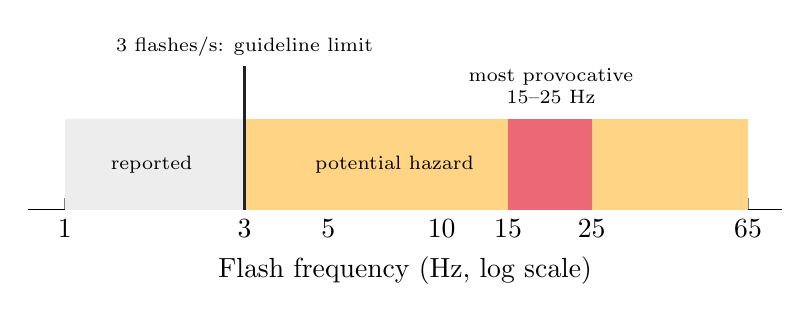
\begin{tikzpicture}
    \begin{axis}[
        width=0.92\linewidth,height=3.6cm,
        xmode=log,xmin=0.8,xmax=80,ymin=0,ymax=1.05,
        xtick={1,3,5,10,15,25,65},xticklabels={1,3,5,10,15,25,65},
        ytick=\empty,axis x line*=bottom,axis y line=none,
        xlabel={Flash frequency (Hz, log scale)},
        clip=false]
      \fill[ink!8] (axis cs:1,0) rectangle (axis cs:65,0.6);
      \fill[hot!55] (axis cs:3,0) rectangle (axis cs:65,0.6);
      \fill[flash!70] (axis cs:15,0) rectangle (axis cs:25,0.6);
      \draw[very thick,ink] (axis cs:3,0) -- (axis cs:3,0.95);
      \node[font=\scriptsize,anchor=south,align=center] at (axis cs:3,0.95) {3 flashes/s: guideline limit};
      \node[font=\scriptsize,align=center] at (axis cs:19.5,0.82) {most provocative\\15--25 Hz};
      \node[font=\scriptsize] at (axis cs:1.7,0.3) {reported};
      \node[font=\scriptsize,align=center] at (axis cs:7.5,0.3) {potential hazard};
    \end{axis}
  \end{tikzpicture}
  \caption{Flash frequency and seizure provocation: a schematic of the ranges reported by the Epilepsy Foundation review~\cite{fisher2005review}. The guidelines draw the line at three flashes, that is six alternating transitions, in any one second.}
  \label{fig:frequency}
\end{figure}

\subsection{From clinical findings to guidelines}

Every guideline reduces these findings to the same three tests (\cref{fig:three}). A sequence is hazardous only when all three hold at once:

\begin{enumerate}
  \item \textbf{Intensity}: each change is large enough. For luminance, a change of 10\% of the maximum relative luminance, with the darker image below 80\%. For colour, a large enough change to or from saturated red.
  \item \textbf{Area}: enough of the field of view changes together.
  \item \textbf{Count}: there are more than three flashes, that is more than six opposing transitions, within any one second.
\end{enumerate}

\begin{figure}[ht]
  \centering
  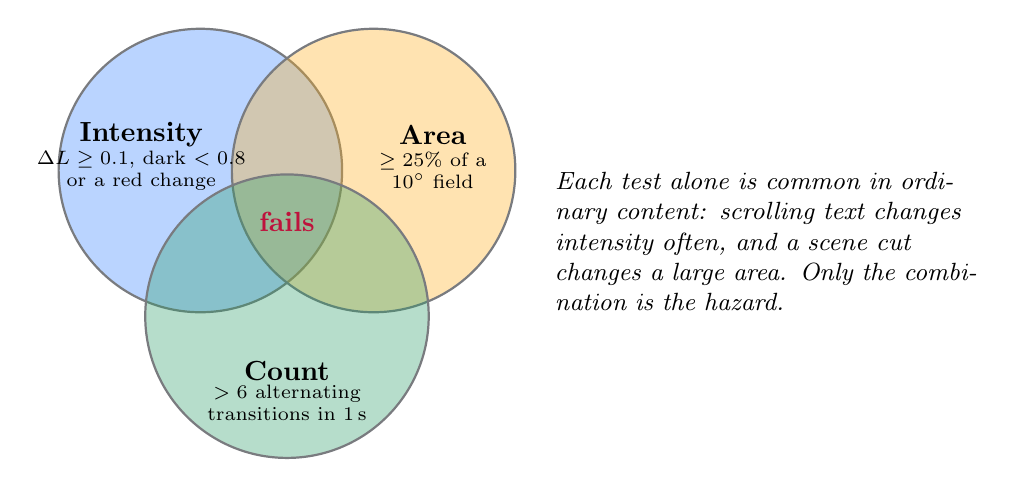
\begin{tikzpicture}[circ/.style={circle,minimum size=3.6cm,draw=ink!60,line width=0.8pt,fill opacity=0.35,text opacity=1}]
    \node[circ,fill=cold] (i) at (0,0) {};
    \node[circ,fill=hot] (a) at (2.2,0) {};
    \node[circ,fill=calm] (c) at (1.1,-1.85) {};
    \node[font=\bfseries] at (-0.75,0.45) {Intensity};
    \node[font=\scriptsize,align=center] at (-0.75,0) {$\Delta L \ge 0.1$, dark $<0.8$\\or a red change};
    \node[font=\bfseries] at (2.95,0.45) {Area};
    \node[font=\scriptsize,align=center] at (2.95,0) {$\ge 25\%$ of a\\\ang{10} field};
    \node[font=\bfseries] at (1.1,-2.55) {Count};
    \node[font=\scriptsize,align=center] at (1.1,-2.95) {$>6$ alternating\\transitions in 1\,s};
    \node[font=\bfseries\color{brandDark},align=center] at (1.1,-0.65) {fails};
    \node[font=\small\itshape,align=left,anchor=west,text width=5.3cm] at (4.4,-0.9)
      {Each test alone is common in ordinary content: scrolling text changes intensity often, and a scene cut changes a large area. Only the combination is the hazard.};
  \end{tikzpicture}
  \caption{The three tests every flash guideline applies. Content fails only where all three overlap.}
  \label{fig:three}
\end{figure}

The guidelines differ mainly in how they measure area. \Cref{tab:guidelines} compares them. WCAG defines the area as a quarter of a \ang{10} visual field. On a reference screen of $1024\times768$ pixels viewed at a typical distance, it equates that field to a rectangle of $341\times256$ pixels, and it counts flashes that happen concurrently and contiguously by their combined area~\cite{wcag22}. \Cref{fig:field} shows the geometry. Broadcast guidance measures a quarter of the whole screen, because a television's viewing distance scales with its size.

\begin{table}[ht]
  \centering\small
  \caption{Flash thresholds in the main guidelines, as implemented by \psv{}'s presets.}
  \label{tab:guidelines}
  \begin{tabularx}{\linewidth}{@{}l>{\raggedright\arraybackslash}X>{\raggedright\arraybackslash}X>{\raggedright\arraybackslash}X@{}}
    \toprule
    & \textbf{WCAG 2.2, SC 2.3.1}~\cite{wcag22} & \textbf{Trace Center, 2024}~\cite{tracemedia} & \textbf{Broadcast}~\cite{itu1702,ofcom,iso9241391} \\
    \midrule
    Luminance change & $\ge 0.1$ relative luminance, darker image $< 0.8$ & as WCAG & \SI{20}{cd/m^2} on a \SI{200}{cd/m^2} display, i.e.\ 0.1 \\
    Red change & saturated red, $\Delta(u',v') \ge 0.2$ & as WCAG & saturated red transitions \\
    Area & 25\% of any $341\times256$ px region & 25\% of any $416\times416$ px region & 25\% of the screen \\
    Count & $>3$ flashes ($>6$ transitions) in 1\,s & as WCAG & as WCAG \\
    \psv{} preset & \code{WCAG22()} (default) & \code{Trace24()} & \code{Broadcast()} \\
    \bottomrule
  \end{tabularx}
\end{table}

\begin{figure}[ht]
  \centering
  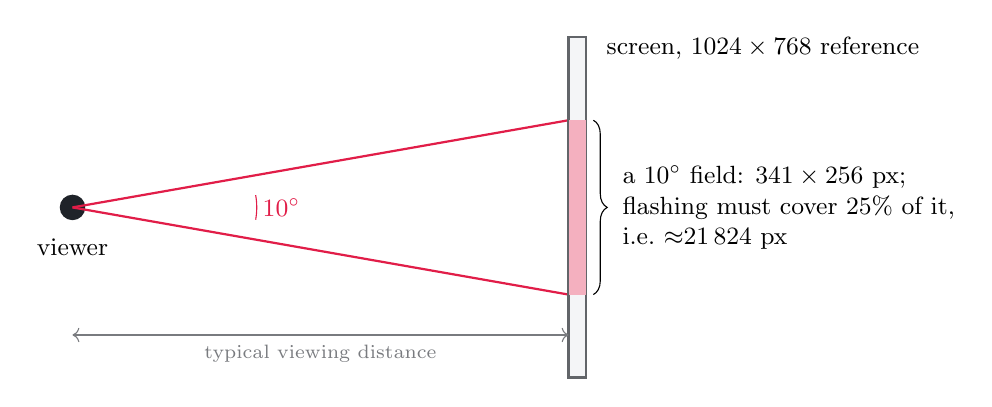
\begin{tikzpicture}[scale=0.9]
    % eye and field
    \fill[ink] (0,0) circle (0.18);
    \draw[thick,brand] (0,0) -- (7,1.23);
    \draw[thick,brand] (0,0) -- (7,-1.23);
    \draw[brand] (1.6,0) ++(10:1) arc (10:-10:1);
    \node[font=\small,brand] at (2.95,0) {\ang{10}};
    \node[font=\small,anchor=north] at (0,-0.3) {viewer};
    % screen
    \draw[thick,ink!70,fill=panel] (7,-2.4) rectangle (7.25,2.4);
    \node[font=\small,anchor=west] at (7.4,2.25) {screen, $1024\times768$ reference};
    \fill[brand!35] (7,-1.23) rectangle (7.25,1.23);
    \draw[decorate,decoration={brace,amplitude=5pt}] (7.35,1.23) -- (7.35,-1.23)
      node[midway,right=7pt,font=\small,align=left] {a \ang{10} field: $341\times256$ px;\\flashing must cover 25\% of it,\\i.e.\ $\approx$\num{21824} px};
    \draw[<->,ink!60] (0,-1.8) -- node[below,font=\scriptsize]{typical viewing distance} (7,-1.8);
  \end{tikzpicture}
  \caption{How WCAG turns a visual angle into pixels. The $341\times256$ rectangle stands for a quarter of the display at a typical viewing distance. \psv{} checks it at every position in the frame, and \guard{} scales it by the display's points per captured pixel.}
  \label{fig:field}
\end{figure}

% ---------------------------------------------------------------- 3
\section{Measuring flashes in pixels: \psv{}}
\label{sec:psv}

\psv{}~\cite{psv} is a Go library and command-line tool that applies these thresholds to every pixel of every frame. Its design goal is to state each guideline as an exact rule on pixels and to apply that rule without approximation, so that a verdict can be traced to the frames, regions and pixels that caused it. This section follows a frame through the detector.

\subsection{From colour values to light}
\label{sec:luminance}

Video and screen pixels are stored as gamma-encoded sRGB values from 0 to 255. Flash thresholds are defined on light, so \psv{} first linearises each channel with the sRGB transfer function~\cite{srgb}:
\begin{equation}
  C_{\text{lin}} =
  \begin{cases}
    C/12.92 & C \le 0.04045,\\[2pt]
    \left(\dfrac{C+0.055}{1.055}\right)^{2.4} & \text{otherwise,}
  \end{cases}
  \qquad C = \frac{\text{value}}{255},
\end{equation}
and computes the relative luminance
\begin{equation}
  L = 0.2126\,R_{\text{lin}} + 0.7152\,G_{\text{lin}} + 0.0722\,B_{\text{lin}} \in [0,1].
  \label{eq:luminance}
\end{equation}
Frames larger than full HD are reduced by an integer factor, averaging blocks of pixels in linear light, so that a bright detail does not vanish into a darker average. \Cref{fig:transfer} shows the transfer curve and the luminance band in which transitions count.

\begin{figure}[ht]
  \centering
  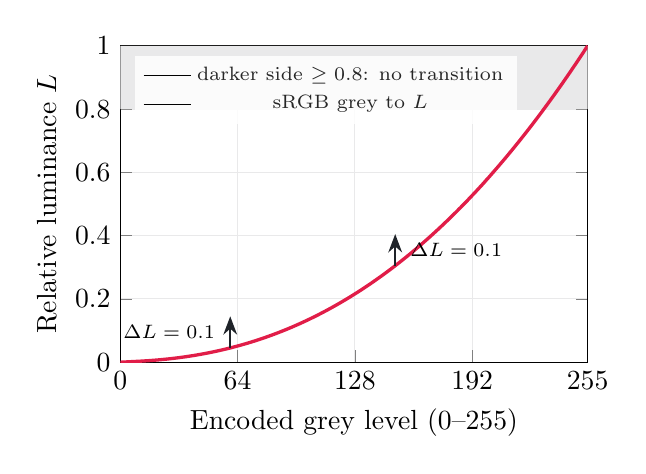
\begin{tikzpicture}
    \begin{axis}[width=0.62\linewidth,height=5.6cm,xmin=0,xmax=255,ymin=0,ymax=1,
        xlabel={Encoded grey level (0--255)},ylabel={Relative luminance $L$},
        xtick={0,64,128,192,255},grid=major,grid style={ink!10},
        legend style={font=\scriptsize,at={(0.03,0.97)},anchor=north west,draw=none,fill=white,fill opacity=0.85}]
      \addplot[name path=top,draw=none,domain=0:255] {1};
      \addplot[name path=dark,draw=none,domain=0:255] {0.8};
      \addplot[fill=ink!10,draw=none,area legend] fill between[of=top and dark];
      \addlegendentry{darker side $\ge 0.8$: no transition}
      \addplot[very thick,brand,domain=0:255,samples=200]
        {(x/255<=0.04045) ? (x/255/12.92) : (((x/255+0.055)/1.055)^2.4)};
      \addlegendentry{sRGB grey to $L$}
      \draw[ink,thick,-{Stealth}] (axis cs:150,0.305) -- (axis cs:150,0.405);
      \node[font=\scriptsize,anchor=west] at (axis cs:153,0.355) {$\Delta L = 0.1$};
      \draw[ink,thick,-{Stealth}] (axis cs:60,0.045) -- (axis cs:60,0.145);
      \node[font=\scriptsize,anchor=east] at (axis cs:57,0.095) {$\Delta L = 0.1$};
    \end{axis}
  \end{tikzpicture}
  \caption{The sRGB transfer function for greys. A change of 0.1 in relative luminance is a much smaller step in encoded values near black than near white, which is why \psv{} works in linear light. Changes whose darker side is above 0.8 (shaded) are not transitions.}
  \label{fig:transfer}
\end{figure}

\subsection{Transitions}

\psv{} compares each pixel with the same pixel in the previous frame and classifies the change as a \emph{step} up, a step down, or no step, for two kinds of flash.

\paragraph{Luminance.} A pixel makes a luminance step between frames $t-1$ and $t$ when
\begin{equation}
  |L_t - L_{t-1}| \ge \Delta L \quad\text{and}\quad \min(L_t, L_{t-1}) < L_{\text{dark}},
  \qquad \Delta L = 0.1,\; L_{\text{dark}} = 0.8 .
\end{equation}

\paragraph{Saturated red.} A pixel is saturated red when red carries at least 80\% of its light, $R_{\text{lin}}/(R_{\text{lin}}+G_{\text{lin}}+B_{\text{lin}}) \ge 0.8$, computed in linear light. (\psv{} found that the Trace Center's red test media only agree with the linear reading~\cite{tracemedia}.) A pixel makes a red step when it is saturated red in one of the two frames and its CIE 1976 chromaticity~\cite{cie015} moves by at least 0.2:
\begin{equation}
  \sqrt{(\Delta u')^2 + (\Delta v')^2} \ge 0.2,\qquad
  u' = \frac{4X}{X+15Y+3Z},\quad v' = \frac{9Y}{X+15Y+3Z}.
\end{equation}
A step into saturated red counts as up and a step out of it as down. Between two saturated reds, a step toward the redder one counts as up. \Cref{fig:uv} places this in the chromaticity diagram. Chromaticity is computed only for pixels that are saturated red in one of the two frames, so ordinary content pays nothing for the red test.

\begin{figure}[ht]
  \centering
  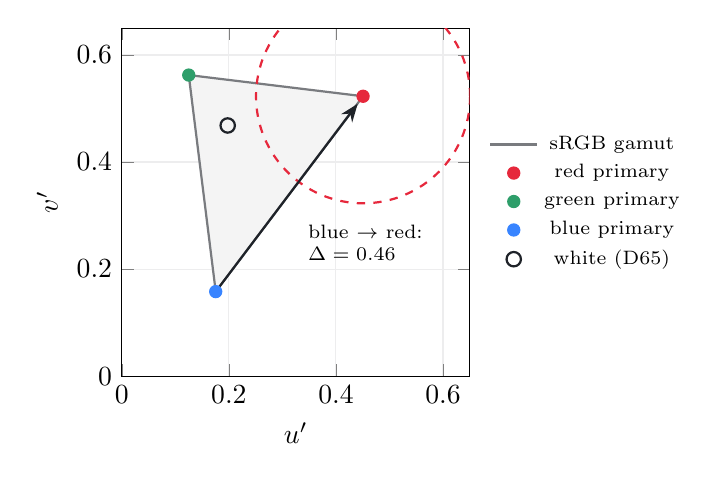
\begin{tikzpicture}
    \begin{axis}[width=0.55\linewidth,height=6cm,xmin=0,xmax=0.65,ymin=0,ymax=0.65,
        xlabel={$u'$},ylabel={$v'$},axis equal image,grid=major,grid style={ink!8},
        legend style={font=\scriptsize,at={(1.03,0.5)},anchor=west,draw=none}]
      \addplot[fill=ink!5,draw=ink!60,thick] coordinates {(0.4507,0.5229) (0.1250,0.5625) (0.1754,0.1579) (0.4507,0.5229)};
      \addlegendentry{sRGB gamut}
      \addplot[only marks,mark=*,mark size=2.2pt,flash] coordinates {(0.4507,0.5229)};
      \addlegendentry{red primary}
      \addplot[only marks,mark=*,mark size=2.2pt,calm] coordinates {(0.1250,0.5625)};
      \addlegendentry{green primary}
      \addplot[only marks,mark=*,mark size=2.2pt,cold] coordinates {(0.1754,0.1579)};
      \addlegendentry{blue primary}
      \addplot[only marks,mark=o,mark size=2.6pt,ink,thick] coordinates {(0.1978,0.4683)};
      \addlegendentry{white (D65)}
      \draw[flash,thick,dashed] (axis cs:0.4507,0.5229) circle [radius=0.2];
      \draw[-{Stealth},thick,ink] (axis cs:0.1754,0.1579) -- (axis cs:0.4407,0.5089);
      \node[font=\scriptsize,anchor=north west,align=left] at (axis cs:0.33,0.30) {blue $\to$ red:\\$\Delta = 0.46$};
    \end{axis}
  \end{tikzpicture}
  \caption{The CIE 1976 $u'v'$ chromaticity of the sRGB primaries. The dashed circle has radius 0.2 around the red primary. A pixel that changes between saturated red and a colour outside that circle, such as the red--blue alternation of the 1997 cartoon, makes a red transition whatever its luminance.}
  \label{fig:uv}
\end{figure}

\subsection{Counting transitions: merging and alternation}

Two rules turn steps into the transitions the guidelines count (\cref{fig:rules}):

\begin{description}[font=\bfseries\color{ink}]
  \item[Steps merge.] A ramp of steps in the same direction on consecutive frames is one transition, counted at its first step. A ramp of steps that are each below the threshold is no transition, even if the total change is larger. A slow fade therefore never counts, however far it goes.
  \item[Transitions alternate.] A transition counts only when it goes the opposite way to the pixel's last counted one. A flash is a pair of opposing transitions, so ``more than three flashes'' becomes \emph{seven or more alternating transitions}.
\end{description}

\begin{figure}[ht]
  \centering
  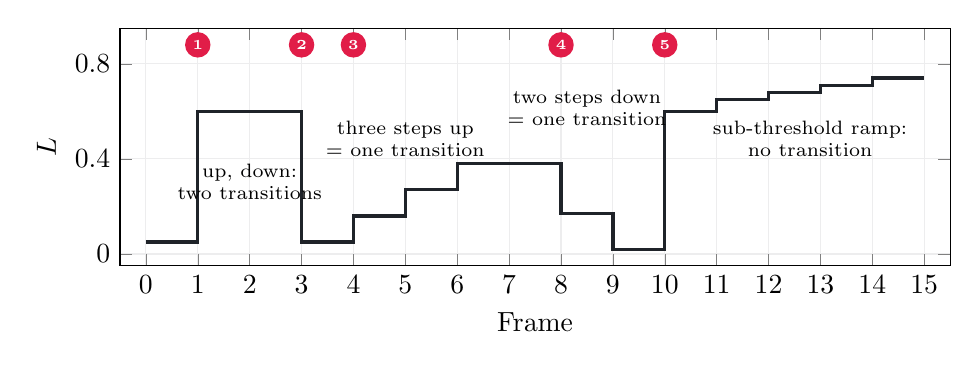
\begin{tikzpicture}
    \begin{axis}[width=\linewidth,height=4.6cm,xmin=-0.5,xmax=15.5,ymin=-0.05,ymax=0.95,
        xlabel={Frame},ylabel={$L$},xtick={0,...,15},ytick={0,0.4,0.8},grid=major,grid style={ink!8},
        clip=false]
      \addplot[const plot,very thick,ink] coordinates {
        (0,0.05) (1,0.6) (2,0.6) (3,0.05) (4,0.16) (5,0.27) (6,0.38) (7,0.38) (8,0.17) (9,0.02) (10,0.6) (11,0.65) (12,0.68) (13,0.71) (14,0.74) (15,0.74)};
      % counted transitions
      \node[circle,fill=brand,text=white,font=\tiny\bfseries,inner sep=1.5pt] at (axis cs:1,0.88) {1};
      \node[circle,fill=brand,text=white,font=\tiny\bfseries,inner sep=1.5pt] at (axis cs:3,0.88) {2};
      \node[circle,fill=brand,text=white,font=\tiny\bfseries,inner sep=1.5pt] at (axis cs:4,0.88) {3};
      \node[circle,fill=brand,text=white,font=\tiny\bfseries,inner sep=1.5pt] at (axis cs:8,0.88) {4};
      \node[circle,fill=brand,text=white,font=\tiny\bfseries,inner sep=1.5pt] at (axis cs:10,0.88) {5};
      \node[font=\scriptsize,align=center,anchor=north] at (axis cs:2,0.42) {up, down:\\two transitions};
      \node[font=\scriptsize,align=center,anchor=south] at (axis cs:5,0.37) {three steps up\\= one transition};
      \node[font=\scriptsize,align=center,anchor=south] at (axis cs:8.5,0.5) {two steps down\\= one transition};
      \node[font=\scriptsize,align=center,anchor=north] at (axis cs:12.8,0.6) {sub-threshold ramp:\\no transition};
    \end{axis}
  \end{tikzpicture}
  \caption{How steps become counted transitions (numbered). Consecutive steps in one direction merge into one transition at the first step. Each counted transition must oppose the previous one. Small steps never count, even when they add up to a large change.}
  \label{fig:rules}
\end{figure}

\Cref{fig:trace} shows the rules at work on two real pixels. The first is the centre of \psv{}'s failing example ``colors-epilepsy-warning''. It cycles green, red and blue on successive frames at \ColorsFPS{}~fps. The step from green to red is a transition down. The step from red to blue is a second step down on the next frame, so it merges into the first. The step back to green is a transition up. The pixel therefore makes two counted transitions every three frames, and its seventh counted transition arrives \SI{\ColorsFirstFail}{\second} into the clip. At that frame the pixel is flashing. The second is a pixel of the synthetic ``localised flash'' clip used throughout this paper: a white box flashing five times a second over dark text. It makes ten transitions a second and reaches seven at \SI{\LocalFirstFail}{\second}.

\pgfplotstableread[col sep=comma]{data/colors-frames.csv}\colorsframes
\pgfplotstableread[col sep=comma]{data/local-frames.csv}\localframes
\begin{figure}[ht]
  \centering
  \begin{tikzpicture}
    \begin{axis}[name=lum1,width=0.5\linewidth,height=4.2cm,xmin=0,xmax=1,ymin=0,ymax=1.05,
        title={\small colors-epilepsy-warning, centre pixel},ylabel={$L$},xticklabels={},
        grid=major,grid style={ink!8}]
      \addplot[const plot,thick,ink] table[x=t,y=lum] {\colorsframes};
      \addplot[only marks,mark=*,mark size=1.7pt,brand] table[x=t,y expr=\thisrow{counted}>0 ? \thisrow{lum} : nan] {\colorsframes};
    \end{axis}
    \begin{axis}[at={(lum1.below south west)},anchor=north west,yshift=-2pt,width=0.5\linewidth,height=3.6cm,
        xmin=0,xmax=1,ymin=0,ymax=24,xlabel={Time (s)},ylabel={count in 1\,s},grid=major,grid style={ink!8}]
      \addplot[const plot,thick,brand] table[x=t,y=recent] {\colorsframes};
      \addplot[dashed,ink,domain=0:1] {6.5};
      \node[font=\scriptsize,anchor=south west] at (axis cs:0.02,6.6) {flashes above 6};
    \end{axis}
    \begin{axis}[name=lum2,at={(lum1.east)},anchor=west,xshift=1.3cm,width=0.5\linewidth,height=4.2cm,xmin=0.8,xmax=2.2,ymin=0,ymax=1.05,
        title={\small localised flash, pixel in the box},xticklabels={},grid=major,grid style={ink!8}]
      \addplot[const plot,thick,ink] table[x=t,y=lum] {\localframes};
      \addplot[only marks,mark=*,mark size=1.7pt,brand] table[x=t,y expr=\thisrow{counted}>0 ? \thisrow{lum} : nan] {\localframes};
    \end{axis}
    \begin{axis}[at={(lum2.below south west)},anchor=north west,yshift=-2pt,width=0.5\linewidth,height=3.6cm,
        xmin=0.8,xmax=2.2,ymin=0,ymax=16,xlabel={Time (s)},grid=major,grid style={ink!8}]
      \addplot[const plot,thick,brand] table[x=t,y=recent] {\localframes};
      \addplot[dashed,ink,domain=0.8:2.2] {6.5};
    \end{axis}
  \end{tikzpicture}
  \caption{Two real pixels traced through \psv{}'s rules. Top: relative luminance, with counted transitions marked. Bottom: the number of counted transitions within the last second. A pixel flashes once the count exceeds six. Left, the green--red--blue cycle merges the red-to-blue step into the transition before it. Right, the localised flash makes one transition per change of the box.}
  \label{fig:trace}
\end{figure}

\subsection{Remembering a second of history in a few words}

Each pixel stores the frames of its counted transitions as a bitmask over the last two seconds: one bit per frame, packed into 64-bit words (\cref{fig:bits}). When a pixel transitions, its mask is shifted by the number of frames since its last update and the newest bit is set. The number of transitions within the last second is then a population count of the newest $r$ bits, where $r=\operatorname{round}(\text{fps})$, so 29.97 fps uses 30. Pixels that do not transition are never touched, so a still frame costs one comparison per pixel.

\begin{figure}[ht]
  \centering
  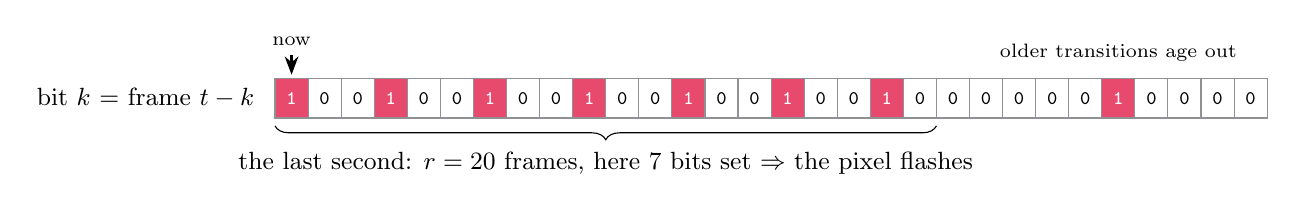
\begin{tikzpicture}[bit/.style={draw=ink!50,minimum width=0.42cm,minimum height=0.5cm,font=\scriptsize\ttfamily,inner sep=0}]
    \foreach \i/\b in {0/1,1/0,2/0,3/1,4/0,5/0,6/1,7/0,8/0,9/1,10/0,11/0,12/1,13/0,14/0,15/1,16/0,17/0,18/1,19/0,20/0,21/0,22/0,23/0,24/0,25/1,26/0,27/0,28/0,29/0}{
      \ifnum\b=1 \node[bit,fill=brand!80,text=white] at (\i*0.42,0) {1};
      \else \node[bit,fill=white] at (\i*0.42,0) {0}; \fi
    }
    \draw[decorate,decoration={brace,amplitude=5pt,mirror}] (-0.21,-0.35) -- (8.19,-0.35)
      node[midway,below=6pt,font=\small] {the last second: $r=20$ frames, here 7 bits set $\Rightarrow$ the pixel flashes};
    \node[font=\small,anchor=east] at (-0.35,0) {bit $k$ = frame $t-k$};
    \draw[-{Stealth},thick] (0,0.55) -- (0,0.3);
    \node[font=\scriptsize,anchor=south] at (0,0.55) {now};
    \node[font=\scriptsize,anchor=south] at (10.5,0.35) {older transitions age out};
  \end{tikzpicture}
  \caption{A pixel's transition history. Counting the transitions in any one-second window is a masked population count, so \psv{} can check every window that contains a frame in constant time.}
  \label{fig:bits}
\end{figure}

\subsection{Flashing together: area}

A single pixel that flashes is not yet a hazard. The guidelines measure the \emph{combined area} of flashes that happen concurrently. \psv{} applies that per frame and per region, in three steps.

\begin{enumerate}
  \item \textbf{Flashing pixels.} A pixel flashes in frame $f$ when it makes more than six alternating transitions within some one-second window that contains $f$. Only flashing pixels count toward the area. Two areas that each flash three times a second, out of step with each other, therefore do not add up to six flashes.
  \item \textbf{Region transitions.} For every region position, $341\times256$ pixels under WCAG, \psv{} counts the flashing pixels that start a transition up in this frame, $U$, and those that start one down, $D$. The region transitions in a direction when that count reaches the area threshold:
  \begin{equation}
    \max(U, D) \ge \frac{A}{100}\,w\,h, \qquad A = 25 .
  \end{equation}
  \item \textbf{Region count.} Each region position keeps its recent transitions. Only a transition opposite to the region's last one counts. A region with more than six alternating transitions within one second fails, and so does the frame.
\end{enumerate}

Checking every position of a $341\times256$ window in a 1080p frame naively would take about \num{1.8e11} additions per frame. \psv{} instead builds a summed-area table~\cite{crow1984} of the up and down planes, $S(x,y)=\sum_{x'<x,\,y'<y} v(x',y')$. The count in any window then takes four look-ups (\cref{fig:sat}):
\begin{equation}
  \sum_{\text{window}} v = S(x_2,y_2) - S(x_1,y_2) - S(x_2,y_1) + S(x_1,y_1).
\end{equation}
The region search runs only in frames where enough flashing pixels transition to reach the threshold at all. It runs in parallel across rows, as do the per-pixel steps across bands of rows.

\begin{figure}[ht]
  \centering
  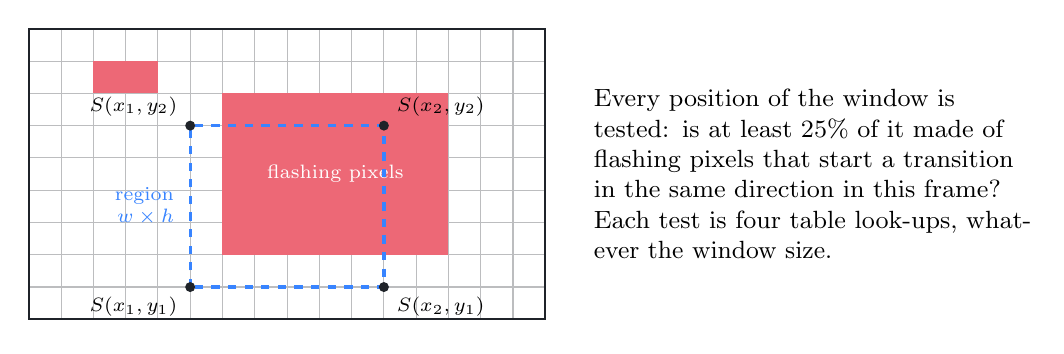
\begin{tikzpicture}[scale=0.82]
    % frame grid
    \draw[ink!30,step=0.5] (0,0) grid (8,4.5);
    \draw[thick,ink] (0,0) rectangle (8,4.5);
    % flashing pixels blob
    \fill[flash!70] (3,1) rectangle (6.5,3.5);
    \fill[flash!70] (1,3.5) rectangle (2,4);
    \node[font=\scriptsize,white] at (4.75,2.25) {flashing pixels};
    % region window
    \draw[very thick,cold,dashed] (2.5,0.5) rectangle (5.5,3);
    \node[font=\scriptsize,cold,anchor=east,align=right] at (2.4,1.75) {region\\$w\times h$};
    % corners
    \foreach \p in {(2.5,0.5),(5.5,0.5),(2.5,3),(5.5,3)} \fill[ink] \p circle (2.2pt);
    \node[font=\scriptsize,anchor=north east] at (2.45,0.5) {$S(x_1,y_1)$};
    \node[font=\scriptsize,anchor=north west] at (5.55,0.5) {$S(x_2,y_1)$};
    \node[font=\scriptsize,anchor=south east] at (2.45,3) {$S(x_1,y_2)$};
    \node[font=\scriptsize,anchor=south west] at (5.55,3) {$S(x_2,y_2)$};
    \node[font=\small,align=left,anchor=west,text width=5.5cm] at (8.6,2.25)
      {Every position of the window is tested: is at least 25\% of it made of flashing pixels that start a transition in the same direction in this frame? Each test is four table look-ups, whatever the window size.};
  \end{tikzpicture}
  \caption{The region search. Flashing pixels that transition up and down in the frame are summed into two tables. A region transitions when either sum over its window reaches a quarter of its area.}
  \label{fig:sat}
\end{figure}

These rules keep apart what the guidelines keep apart. Two halves of an area that flash in sync combine into one area. If one transition of one half is a single frame late, the region misses that transition, because neither half covers the area alone in either frame. Moving patterns, in which every pixel flashes fast but neighbours are a frame or two out of phase, still fail, because in each frame enough of them transition together.

\subsection{Deciding takes a second; flashing does not}

Whether a pixel flashes in frame $f$ depends on every one-second window that contains $f$, including the second \emph{after} it. A frame is therefore \emph{decided} only once $r-1$ more frames have been seen (\cref{fig:delay}). For a finished video, that delay is invisible. For a live screen, a second is far too long: a viewer would see the whole first second of a failing sequence before anyone could act.

The asymmetry that makes live protection possible is this: \emph{only the absence of flashing needs the second after}. Once a pixel has made more than six transitions within the second ending at the current frame, later frames can only add to them, so the pixel flashes whatever comes next. \psv{}'s live mode, \code{Analyzer.Watch}, reports that fact in the frame in which it happens. It also reports how far every other transitioning pixel is from it.

\begin{figure}[ht]
  \centering
  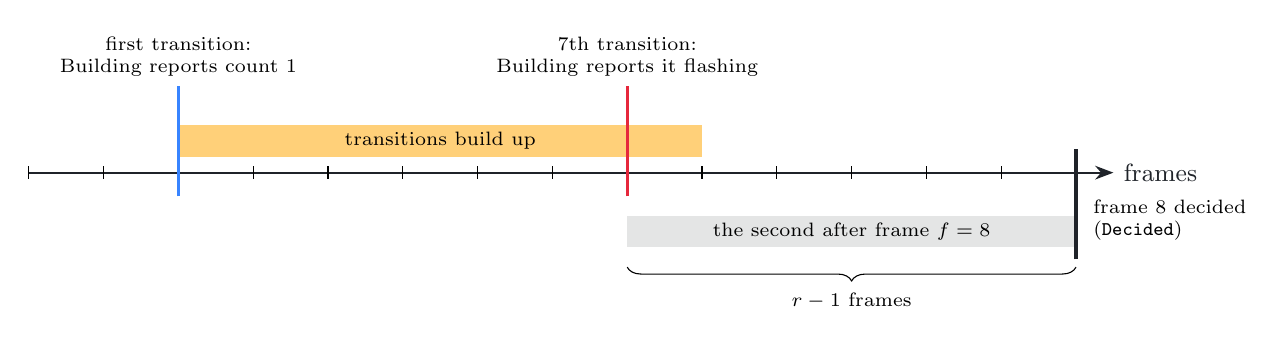
\begin{tikzpicture}[x=0.95cm]
    \draw[-{Stealth},thick,ink] (0,0) -- (14.5,0) node[right,font=\small]{frames};
    \foreach \x in {0,...,14} \draw (\x,0.08) -- (\x,-0.08);
    \fill[hot!60] (2,0.2) rectangle (9,0.6);
    \node[font=\scriptsize] at (5.5,0.4) {transitions build up};
    \draw[very thick,flash] (8,-0.3) -- (8,1.1);
    \node[font=\scriptsize,align=center,anchor=south] at (8,1.1) {7th transition:\\Building reports it flashing};
    \draw[very thick,cold] (2,-0.3) -- (2,1.1);
    \node[font=\scriptsize,align=center,anchor=south] at (2,1.1) {first transition:\\Building reports count 1};
    \fill[ink!12] (8,-0.95) rectangle (14,-0.55);
    \node[font=\scriptsize] at (11,-0.75) {the second after frame $f=8$};
    \draw[very thick,ink] (14,-1.1) -- (14,0.3);
    \node[font=\scriptsize,align=left,anchor=west] at (14.1,-0.6) {frame 8 decided\\(\code{Decided})};
    \draw[decorate,decoration={brace,amplitude=5pt,mirror}] (8,-1.2) -- (14,-1.2) node[midway,below=6pt,font=\scriptsize]{$r-1$ frames};
  \end{tikzpicture}
  \caption{When \psv{} knows what. A pixel's flashing is known in the frame that completes it (\code{Building}). The verdict that a frame passes or fails arrives $r-1$ frames later (\code{Decided}), identical to the offline analysis.}
  \label{fig:delay}
\end{figure}

\subsection{The live measurement: \code{Building}}

For every watched frame, \code{Watch} returns an update with two parts. \code{Decided} holds the frames decided by this one, about a second behind and identical to an offline analysis. \code{Building} measures the frame being watched. Let $T_t$ be the pixels that start a counted transition in frame $t$, $n_i(t)$ the number of transitions pixel $i$ made within the last second, $N$ the number of pixels and $M=6$. For each kind of flash:
\begin{align}
  \text{Peak}_t &= \max_{i\in T_t} n_i(t), &
  \text{Area}_t &= 100\,\frac{|T_t|}{N}, \\
  \text{Flashing}_t &= 100\,\frac{|\{i\in T_t : n_i(t) > M\}|}{N}, &
  \text{Mask}_t[c] &= \max_{i\in T_t\cap c} n_i(t),
\end{align}
where $c$ ranges over the cells of a $64\times36$ grid laid over the frame. \code{Building} is provisional and pixel-level. It applies no area threshold and no direction, so it also reports flashing that is too small to fail. Its \code{Flashing} pixels, however, are final: they count as flashing in the decided result. Measuring it costs one population count per transitioning pixel.

\Cref{fig:building} shows the mask during the localised flash. The box is blue at its second transition, amber at its fourth, and red at its seventh, when \psv{} reports it flashing. One second after that frame, \psv{} decides the failure and reports the share of each cell that flashed (\cref{fig:building}d).

\begin{figure}[htbp]
  \centering
  \begin{subfigure}{0.49\linewidth}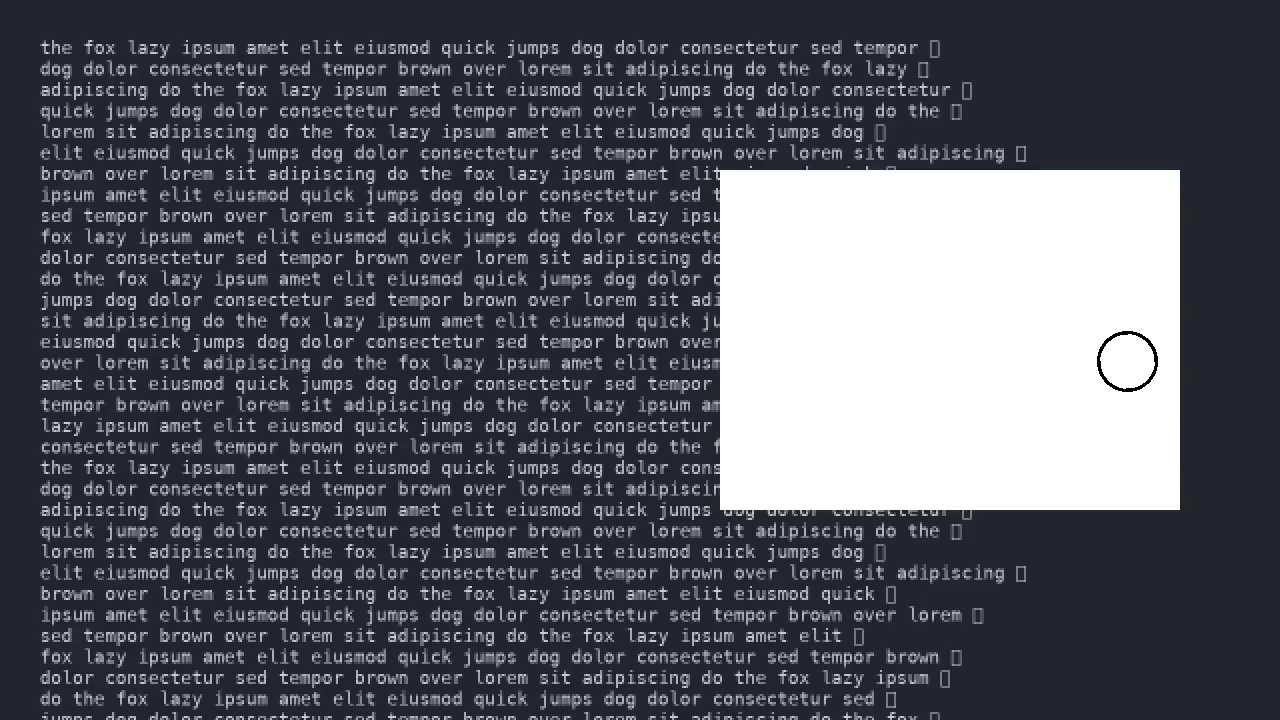
\includegraphics[width=\linewidth]{local-frame.png}\caption{The clip: a box flashing 5 times a second over text. The ring marks the pixel of \cref{fig:trace}.}\end{subfigure}\hfill
  \begin{subfigure}{0.49\linewidth}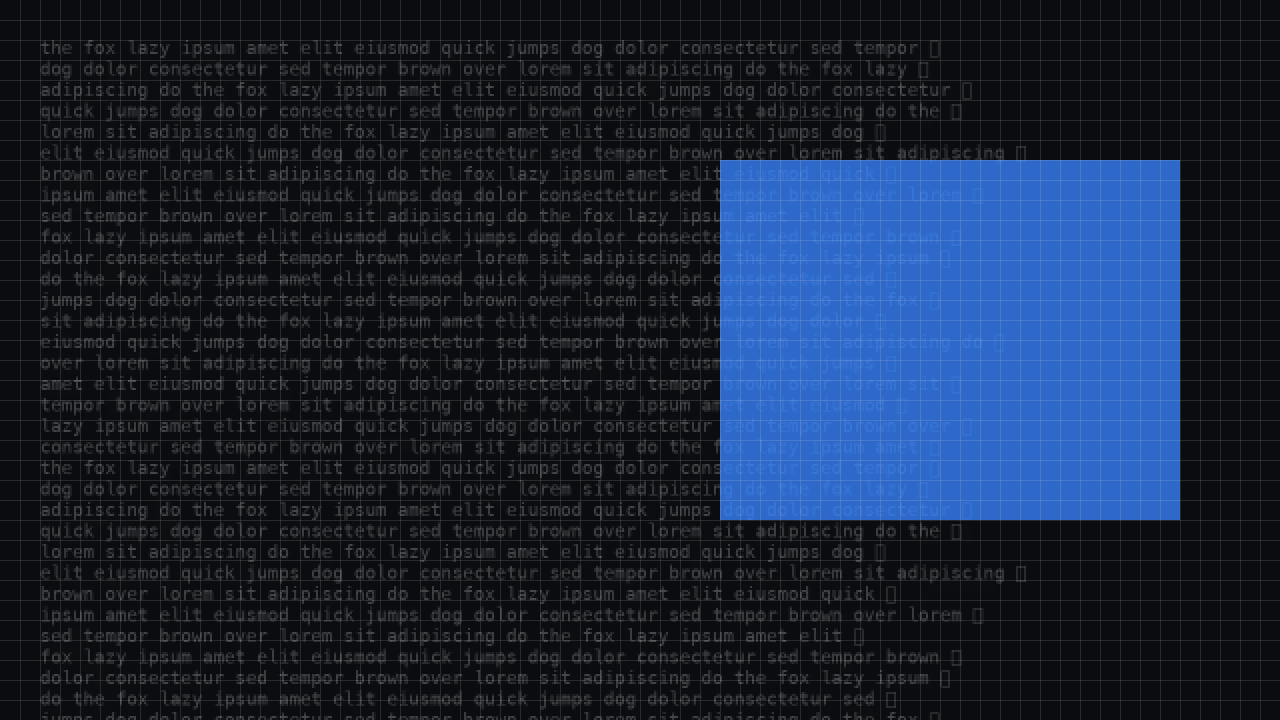
\includegraphics[width=\linewidth]{local-building-a.png}\caption{\code{Building.Mask} at \SI{\SnapLocala}{\second}: 2 transitions.}\end{subfigure}\\[4pt]
  \begin{subfigure}{0.49\linewidth}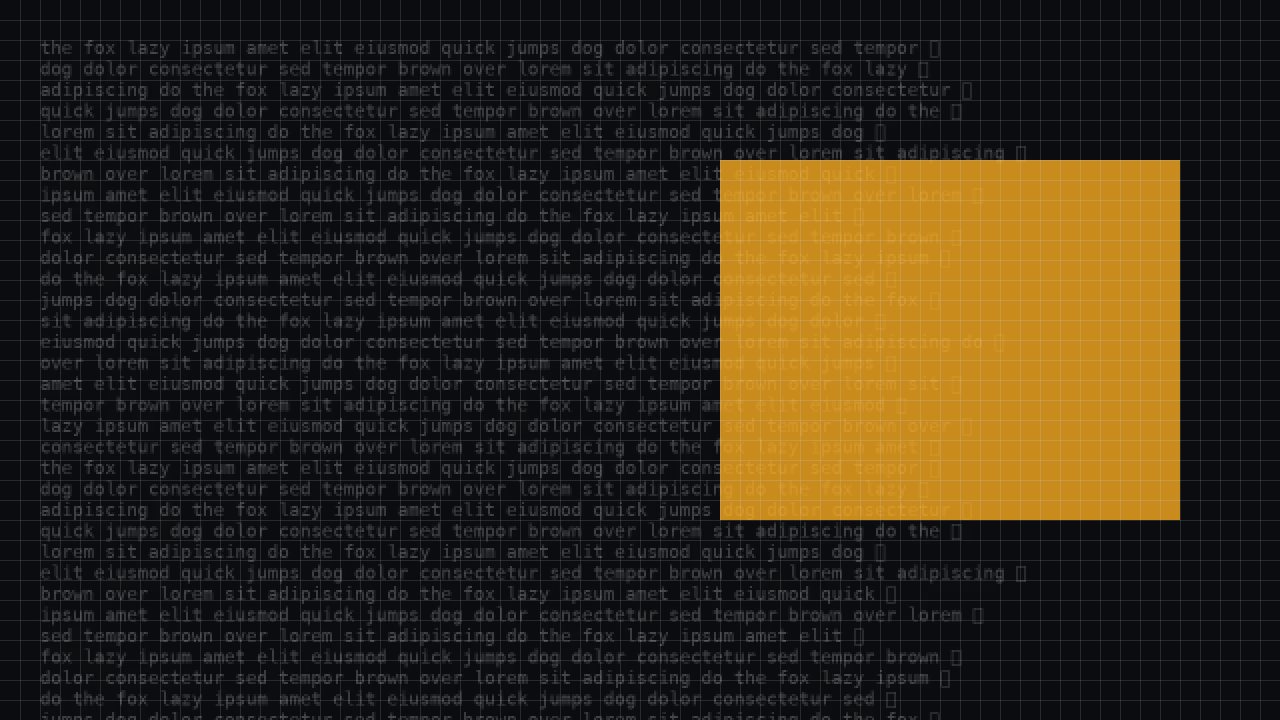
\includegraphics[width=\linewidth]{local-building-b.png}\caption{At \SI{\SnapLocalb}{\second}: 4 transitions; the cells are \emph{hot}.}\end{subfigure}\hfill
  \begin{subfigure}{0.49\linewidth}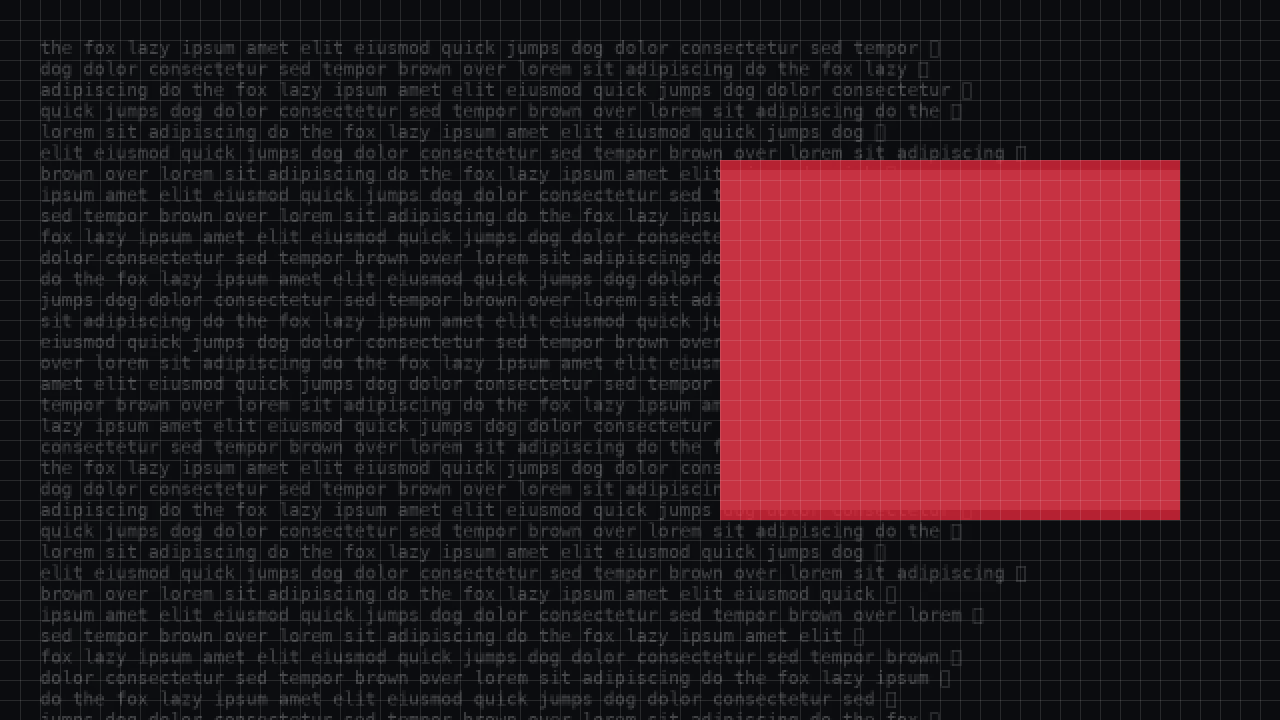
\includegraphics[width=\linewidth]{local-building-c.png}\caption{At \SI{\SnapLocalc}{\second}: 7 transitions; the pixels flash.}\end{subfigure}\\[4pt]
  \begin{subfigure}{0.49\linewidth}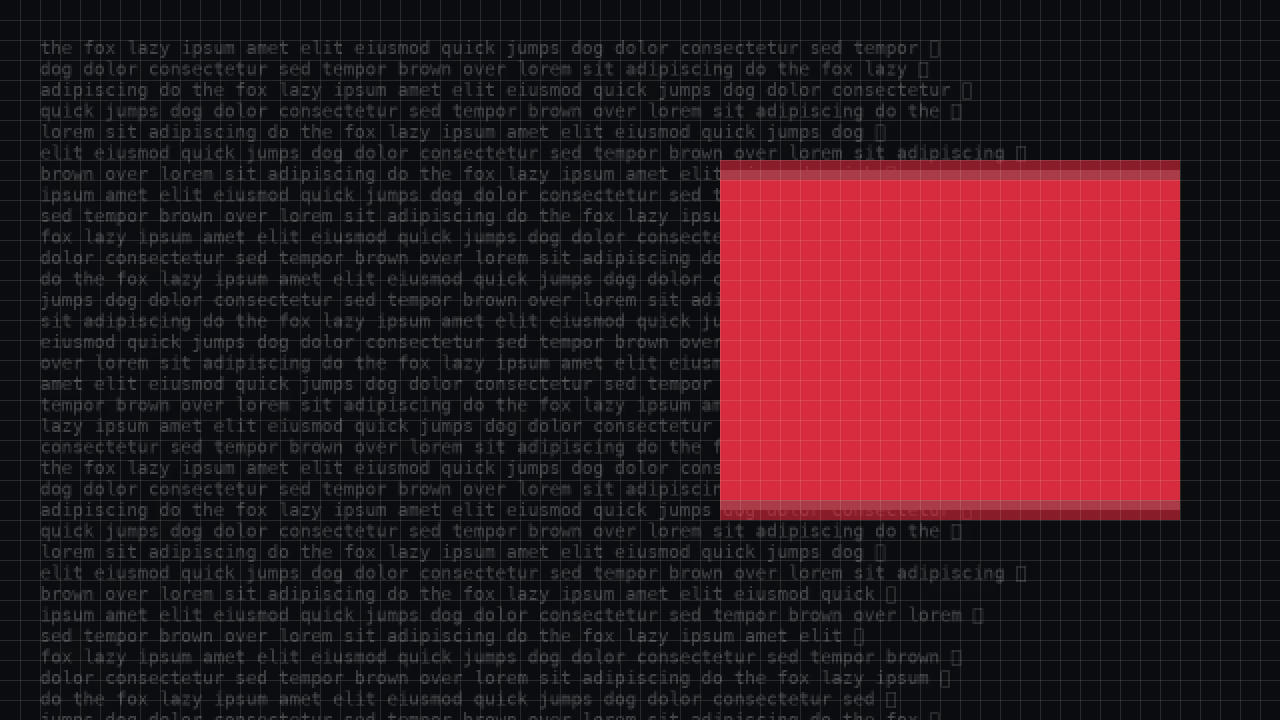
\includegraphics[width=\linewidth]{local-decided.png}\caption{\code{Decided} for the frame at \SI{\LocalFirstFail}{\second}: share of each cell that flashed.}\end{subfigure}\hfill
  \begin{subfigure}{0.49\linewidth}\centering
    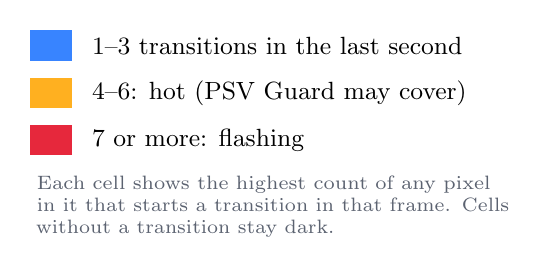
\begin{tikzpicture}[sw/.style={minimum width=0.55cm,minimum height=0.4cm,draw=white}]
      \node[sw,fill=cold] (a) at (0,1.5) {}; \node[anchor=west,font=\small] at (0.4,1.5) {1--3 transitions in the last second};
      \node[sw,fill=hot] (b) at (0,0.9) {}; \node[anchor=west,font=\small] at (0.4,0.9) {4--6: hot (\guard{} may cover)};
      \node[sw,fill=flash] (c) at (0,0.3) {}; \node[anchor=west,font=\small] at (0.4,0.3) {7 or more: flashing};
      \node[anchor=west,font=\scriptsize,text width=6cm,color=muted] at (-0.3,-0.55) {Each cell shows the highest count of any pixel in it that starts a transition in that frame. Cells without a transition stay dark.};
    \end{tikzpicture}\caption{Key.}\end{subfigure}
  \caption{\psv{}'s live measurement during the localised flash, on the $64\times36$ grid. All images are produced by \psv{} from the clip; nothing is drawn by hand.}
  \label{fig:building}
\end{figure}

\Cref{fig:buildingtime} plots \code{Building} over time for both clips, together with the frames \psv{} later decides as failing.

\pgfplotstableread[col sep=comma]{data/colors-ticks.csv}\colorsticks
\pgfplotstableread[col sep=comma]{data/local-ticks.csv}\localticks
\begin{figure}[ht]
  \centering
  \begin{tikzpicture}
    \begin{axis}[name=b1,width=0.52\linewidth,height=5cm,xmin=0,xmax=1.5,ymin=0,ymax=105,
        title={\small colors-epilepsy-warning},xlabel={Time (s)},ylabel={\% of frame},
        grid=major,grid style={ink!8},legend style={font=\scriptsize,at={(0.98,0.4)},anchor=east,fill=white,fill opacity=0.9,draw=none}]
      \addplot[ycomb,flash!35,line width=1.2pt] table[x=t,y expr=\thisrow{failed}>0 ? 100 : nan] {\colorsframes};
      \addlegendentry{decided failing}
      \addplot[only marks,mark=*,mark size=1.6pt,ink] table[x=t,y expr=\thisrow{area}>0 ? \thisrow{area} : nan] {\colorsframes};
      \addlegendentry{Area}
      \addplot[only marks,mark=square*,mark size=1.1pt,brand] table[x=t,y expr=\thisrow{flashing}>0 ? \thisrow{flashing} : nan] {\colorsframes};
      \addlegendentry{Flashing}
    \end{axis}
    \begin{axis}[at={(b1.east)},anchor=west,xshift=1.1cm,width=0.52\linewidth,height=5cm,xmin=0.8,xmax=2.6,ymin=0,ymax=40,
        title={\small localised flash},xlabel={Time (s)},grid=major,grid style={ink!8}]
      \addplot[ycomb,flash!35,line width=1.2pt] table[x=t,y expr=\thisrow{failed}>0 ? 40 : nan] {\localframes};
      \addplot[only marks,mark=*,mark size=1.6pt,ink] table[x=t,y expr=\thisrow{area}>0 ? \thisrow{area} : nan] {\localframes};
      \addplot[only marks,mark=square*,mark size=1.1pt,brand] table[x=t,y expr=\thisrow{flashing}>0 ? \thisrow{flashing} : nan] {\localframes};
    \end{axis}
  \end{tikzpicture}
  \caption{\code{Building} over time. Dots mark frames in which pixels start a transition (Area), squares those of them already flashing (Flashing). Light bars mark the frames \psv{} decides as failing, a second later. The colour example flashes the whole frame from the start. The localised box covers 17\% of the frame.}
  \label{fig:buildingtime}
\end{figure}

\subsection{Performance}

A 1080p frame has two million pixels, and strobe footage can make most of them transition at once. \psv{} keeps exact analysis fast by splitting each frame into row bands analysed in parallel, computing chromaticity only for red candidates, updating histories only for pixels that transition, and running the region search only when the area threshold can be reached. Its documentation reports that a 61-second 1080p strobe clip analyses in about 16 seconds on a 10-core laptop~\cite{psv}. For live use, \guard{} analyses each display at about 640 pixels wide, where one \code{Watch} call took 0.5--6\,ms in the runs reported here.

% ---------------------------------------------------------------- 4
\section{From detection to protection: \guard{}}
\label{sec:guard}

\subsection{Architecture}

\guard{}~\cite{psvguard} is written in Go, with thin Objective-C bindings to ScreenCaptureKit, AppKit and Core Animation (\cref{fig:arch}). Each display has its own capture stream and its own \psv{} analyser. Frames are converted from BGRA straight into pooled \psv{} frames, honouring the row stride, with no per-frame allocation. A fixed-rate resampler presents the analyser with exactly 60 frames per second: the screen only delivers frames when something changes, and \psv{}'s counts assume a constant rate. When the resampler falls behind, it drops the older frame rather than queueing, and every drop is counted.

\begin{figure}[ht]
  \centering
  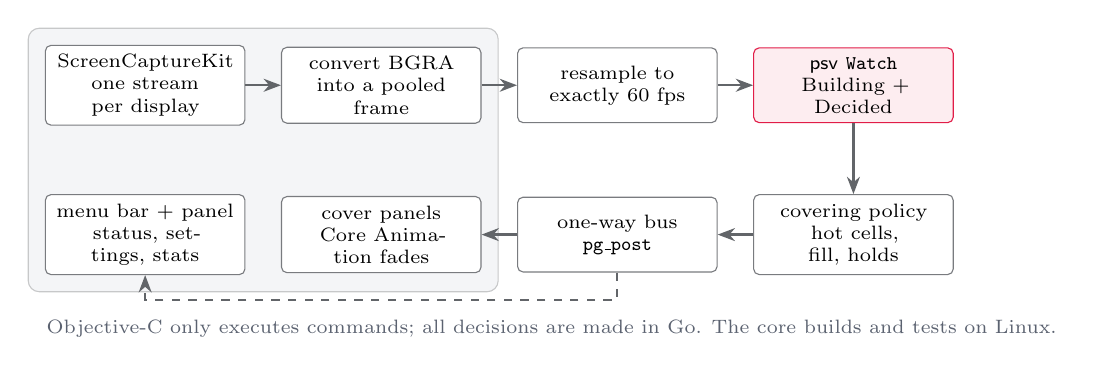
\begin{tikzpicture}[
      blk/.style={draw=ink!60,rounded corners=2pt,fill=white,minimum height=0.95cm,text width=2.3cm,align=center,font=\scriptsize},
      lane/.style={draw=ink!25,fill=panel,rounded corners=4pt},
      arr/.style={-{Stealth[length=2.2mm]},thick,ink!70}]
    \node[blk] (sck) {ScreenCaptureKit\\one stream per display};
    \node[blk,right=0.45cm of sck] (conv) {convert BGRA\\into a pooled frame};
    \node[blk,right=0.45cm of conv] (res) {resample to\\exactly 60 fps};
    \node[blk,right=0.45cm of res,draw=brand,fill=brand!8] (watch) {\psv{} \code{Watch}\\Building + Decided};
    \node[blk,below=0.9cm of watch] (pol) {covering policy\\hot cells, fill, holds};
    \node[blk,left=0.45cm of pol] (bus) {one-way bus\\\code{pg\_post}};
    \node[blk,left=0.45cm of bus] (ov) {cover panels\\Core Animation fades};
    \node[blk,left=0.45cm of ov] (ui) {menu bar + panel\\status, settings, stats};
    \draw[arr] (sck) -- (conv); \draw[arr] (conv) -- (res); \draw[arr] (res) -- (watch);
    \draw[arr] (watch) -- (pol); \draw[arr] (pol) -- (bus); \draw[arr] (bus) -- (ov);
    \draw[arr,dashed] (bus.south) -- ++(0,-0.35) -| (ui.south);
    \begin{scope}[on background layer]
      \node[lane,fit=(sck)(ov)(ui),inner sep=6pt] {};
    \end{scope}
    \node[font=\scriptsize,color=muted,anchor=north west] at ($(ui.south west)+(-0.1,-0.45)$)
      {Objective-C only executes commands; all decisions are made in Go. The core builds and tests on Linux.};
  \end{tikzpicture}
  \caption{\guard{}'s pipeline for one display. Native callbacks only copy and enqueue, the main thread is never blocked, and covers are excluded from the capture so they never feed back into analysis.}
  \label{fig:arch}
\end{figure}

\psv{}'s region size is defined in reference pixels: WCAG's CSS pixels, which are points on macOS. \guard{} captures each display at about 640 pixels wide, so it scales the $341\times256$ region by the captured pixels per point. On a 1728-point-wide display, the region becomes $126\times95$ captured pixels.

\subsection{Why the obvious rule fails}
\label{sec:obvious}

\code{Building} reports, in every frame, which cells contain pixels on their way to flashing. The obvious rule is to cover every cell whose peak reaches a safety margin below the limit, say four transitions: a \emph{hot} cell. That rule covers flashing early. It also covers far too much.

Moving detail makes individual pixels transition constantly. When text scrolls, each glyph edge passes over a pixel and changes its luminance by far more than 0.1, so each pixel steps up and down every few frames. \Cref{fig:scroll} shows the mask for fast-scrolling text: within \SI{\SnapScrollc}{\second}, pixels across the whole page reach seven transitions. By the pixel count alone, they flash. \psv{}'s decided verdict for this clip is a pass, because in no frame do 25\% of any region transition in the same direction. Neighbouring pixels step at different times. The passing advertisement in \psv{}'s examples behaves similarly: film grain and the edges of moving objects put isolated pixels over the count. In early experiments, a plain peak-and-area rule covered that advertisement for its whole length, covered scrolling text within 70\,ms to 1.2\,s, and covered macOS's full-screen animation.

\begin{figure}[ht]
  \centering
  \begin{subfigure}{0.325\linewidth}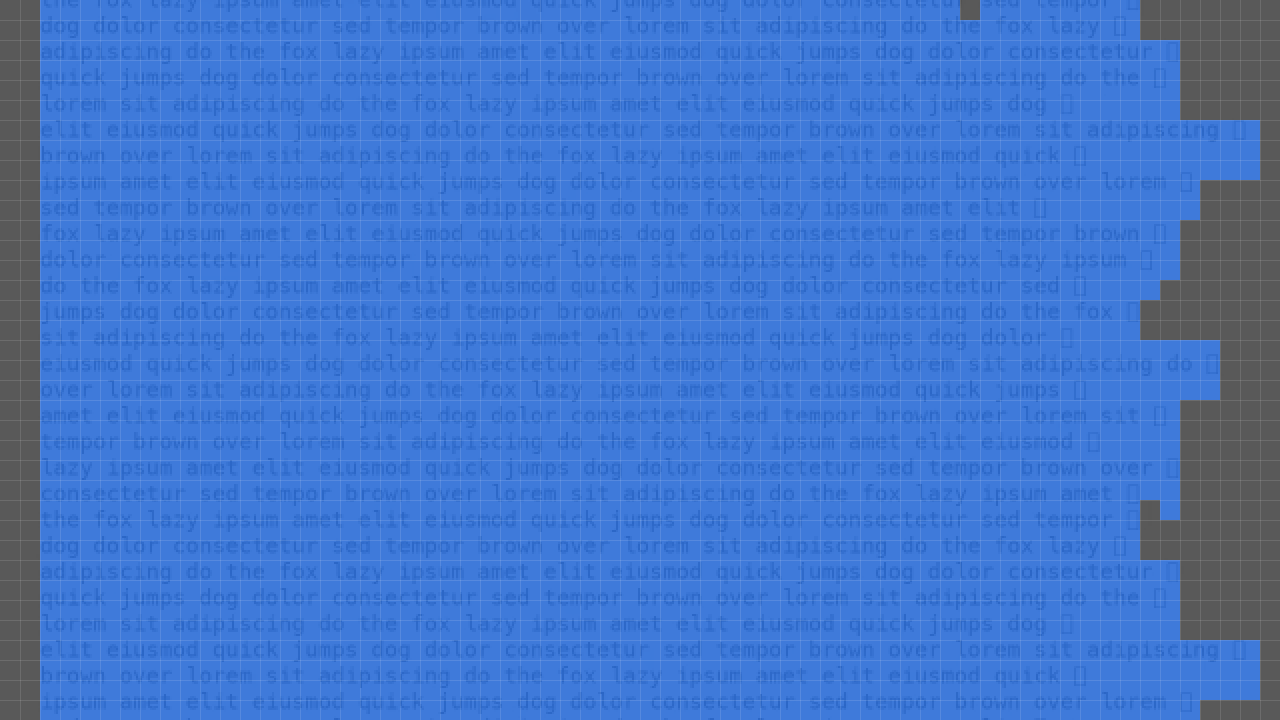
\includegraphics[width=\linewidth]{scroll-building-a.png}\caption{\SI{\SnapScrolla}{\second}: count 2}\end{subfigure}\hfill
  \begin{subfigure}{0.325\linewidth}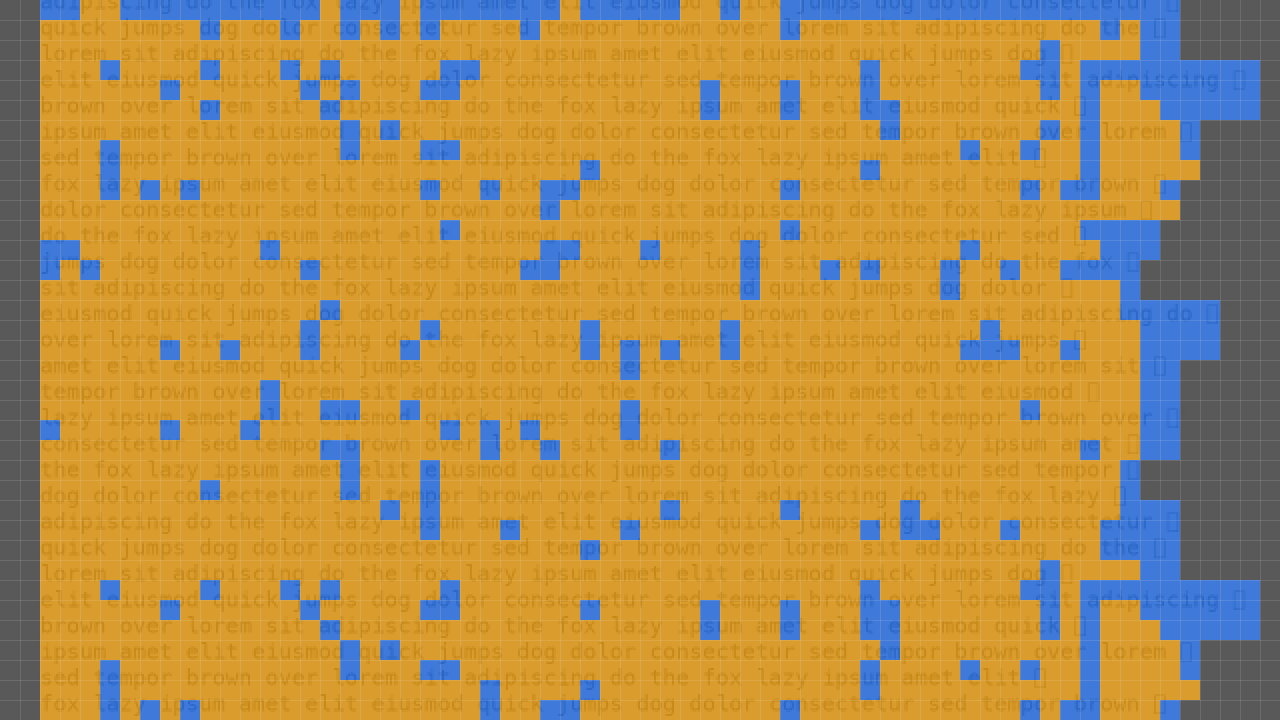
\includegraphics[width=\linewidth]{scroll-building-b.png}\caption{\SI{\SnapScrollb}{\second}: count 4}\end{subfigure}\hfill
  \begin{subfigure}{0.325\linewidth}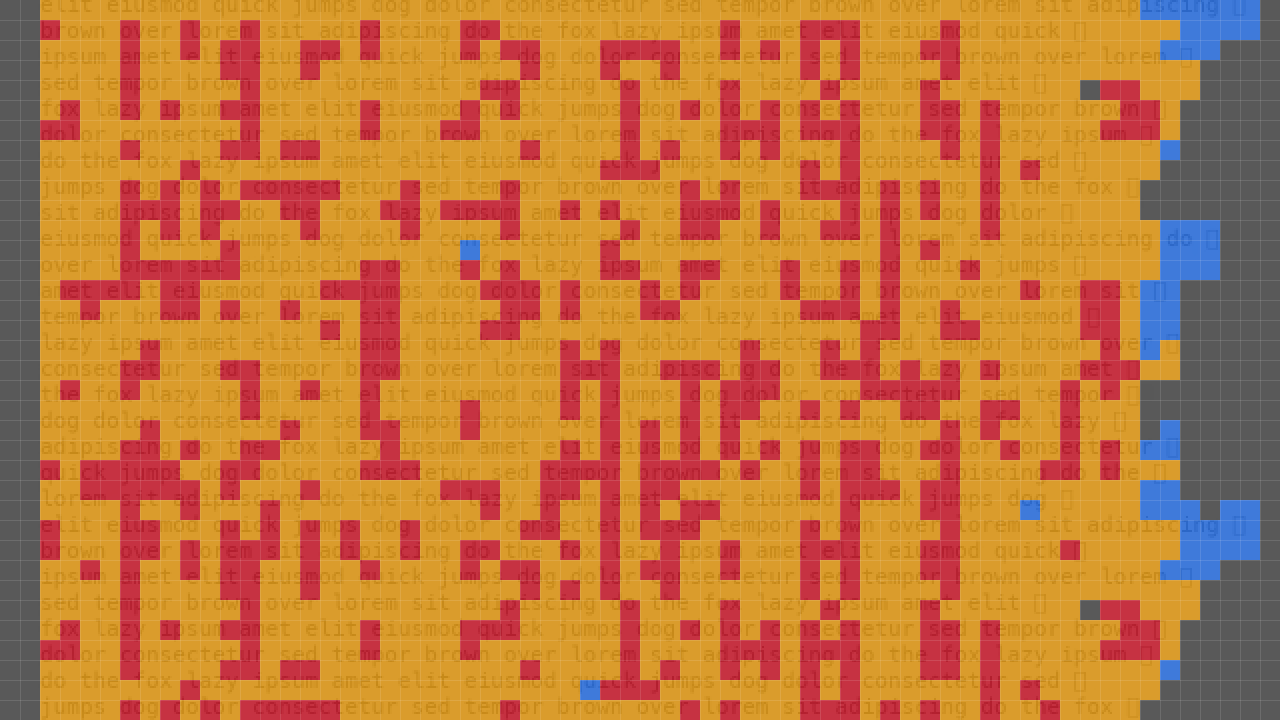
\includegraphics[width=\linewidth]{scroll-building-c.png}\caption{\SI{\SnapScrollc}{\second}: count 7}\end{subfigure}
  \caption{\code{Building.Mask} for text scrolling at 1500 pixels a second. Pixel counts reach the flash limit across the page within a tenth of a second, yet \psv{} decides that the clip passes. The pixel count alone cannot tell flashing from moving detail.}
  \label{fig:scroll}
\end{figure}

\subsection{Fill: does the whole cell change together?}

What separates the two cases is visible in \code{Building} itself. Flashing changes \emph{whole areas} at once. Moving detail changes a scattered fraction of the pixels in each cell it touches. We define the \emph{fill} of a frame as the share of the display that transitions, divided by the share of mask cells that contain any transition:
\begin{equation}
  \text{fill}_t = \frac{\max(\text{Area}^{\text{lum}}_t,\, \text{Area}^{\text{red}}_t)}{100\cdot|\{c : \text{Mask}_t[c] > 0\}| / (64\cdot 36)} .
\end{equation}
A frame in which every pixel of every active cell transitions has a fill of 1. Scattered glyph edges give a fill of about 0.3. \Cref{fig:fill} shows fill per analysed frame for the localised flash, the scrolling text and the passing advertisement. Of the frames with any transition, 97\% of the localised flash's frames have a fill of at least 0.5, against none of the scrolling text's and 7\% of the advertisement's.

\pgfplotstableread[col sep=comma]{data/scroll-ticks.csv}\scrollticks
\pgfplotstableread[col sep=comma]{data/ad-ticks.csv}\adticks
\begin{figure}[ht]
  \centering
  \begin{tikzpicture}
    \begin{axis}[width=\linewidth,height=5.2cm,xmin=0,xmax=4,ymin=0,ymax=1.1,
        xlabel={Time (s)},ylabel={Fill},grid=major,grid style={ink!8},
        legend style={font=\scriptsize,at={(0.99,0.62)},anchor=east,fill=white,fill opacity=0.9,draw=none}]
      \addplot[only marks,mark=*,mark size=1.6pt,flash] table[x=t,y expr=\thisrow{fill}>0 ? \thisrow{fill} : nan] {\localticks};
      \addlegendentry{localised flash (fails)}
      \addplot[only marks,mark=triangle*,mark size=1.4pt,cold] table[x=t,y expr=\thisrow{fill}>0 ? \thisrow{fill} : nan] {\scrollticks};
      \addlegendentry{scrolling text (passes)}
      \addplot[only marks,mark=diamond*,mark size=1.4pt,calm] table[x=t,y expr=\thisrow{fill}>0 ? \thisrow{fill} : nan] {\adticks};
      \addlegendentry{advertisement (passes)}
      \addplot[dashed,thick,ink,domain=0:4] {0.5};
      \node[font=\scriptsize,anchor=south east] at (axis cs:3.98,0.5) {MinFill $=0.5$};
    \end{axis}
  \end{tikzpicture}
  \caption{Fill in each analysed frame with any transition. Flashing fills the cells it touches. Moving text and video detail fill only part of them, with occasional frames above 0.5 when the capture skips a step. The share requirement absorbs those.}
  \label{fig:fill}
\end{figure}

\subsection{The covering policy}

\guard{}'s policy (\cref{fig:policy}) combines the hot-cell mask with fill, a hold time and \psv{}'s decided verdict as a backstop. With the default settings:

\begin{description}[font=\bfseries\color{ink}]
  \item[Hot.] A cell is hot when its peak, luminance or red, is at least 4. Each hot cell is grown by a margin of one cell.
  \item[Start.] Covering starts when hot cells cover at least 15\% of the display, and the fill test passes. Within the last second, at least 2 frames had a fill of at least 0.5, and those were at least 30\% of the frames with any transition (counting at least 8).
  \item[Keep.] An existing cover stays while hot cells continue, and either the fill test still passes or \psv{} reports at least 1\% of the display already flashing. While keeping, covers may only refresh cells already covered or next to them, so a cover cannot creep across moving detail.
  \item[Hold.] Each covered cell stays covered for 3\,s after it was last hot, through the gaps between flashes.
  \item[Whole display.] Once 40\% of a display is covered, the whole display is covered.
  \item[Backstop.] A frame that \psv{} decides as failing, but that was not covered when it was shown, is counted as a \emph{miss}. Its decided mask is covered immediately.
  \item[System transitions.] When macOS switches Spaces, covers begun within the last second are withdrawn, unless forced by the backstop. Fill history is cleared, and no cover starts for 0.6\,s. Space animations sweep the whole screen and can look like a flash.
\end{description}

\begin{figure}[ht]
  \centering
  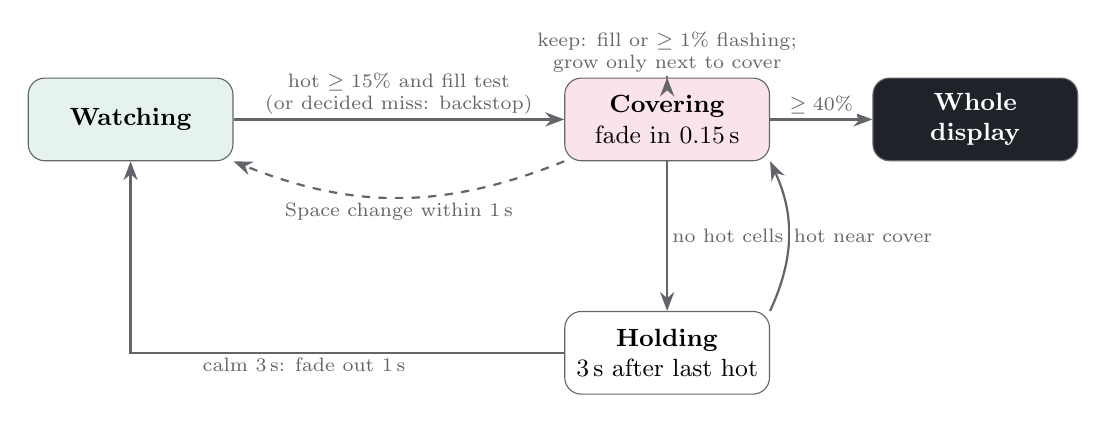
\begin{tikzpicture}[
      st/.style={draw=ink!70,rounded corners=6pt,minimum width=2.6cm,minimum height=1.05cm,align=center,font=\small,fill=white},
      arr/.style={-{Stealth[length=2.4mm]},thick,ink!70},lab/.style={font=\scriptsize,align=center,fill=white,inner sep=1.5pt}]
    \node[st,fill=calm!12] (watch) {\textbf{Watching}};
    \node[st,fill=brand!12,right=4.2cm of watch] (cov) {\textbf{Covering}\\fade in 0.15\,s};
    \node[st,below=1.9cm of cov] (hold) {\textbf{Holding}\\3\,s after last hot};
    \node[st,fill=ink,text=white,right=1.3cm of cov] (full) {\textbf{Whole}\\\textbf{display}};
    \draw[arr] (watch) -- node[lab,above]{hot $\ge 15\%$ and fill test\\(or decided miss: backstop)} (cov);
    \draw[arr] (cov) -- node[lab,right]{no hot cells} (hold);
    \draw[arr] (hold.west) -| node[lab,pos=0.3,below]{calm 3\,s: fade out 1\,s} (watch.south);
    \draw[arr] (hold.north east) to[bend right=25] node[lab,right]{hot near cover} (cov.south east);
    \draw[arr] (cov) -- node[lab,above]{$\ge 40\%$} (full);
    \draw[arr] (cov.north) to[out=60,in=120,looseness=5] node[lab,above]{keep: fill or $\ge 1\%$ flashing;\\grow only next to cover} (cov.north);
    \draw[arr,dashed] (cov.south west) to[bend left=22] node[lab,below]{Space change within 1\,s} (watch.south east);
  \end{tikzpicture}
  \caption{The covering policy for one display. Covers fade in over 0.15\,s and out over 1\,s, and holds prevent rapid toggling, so a cover can never itself become a flashing stimulus.}
  \label{fig:policy}
\end{figure}

\subsection{A frame-by-frame account}

\Cref{fig:timeline} replays the localised flash through \guard{}'s pipeline at 60 frames per second, exactly as captured frames arrive. The box first appears at \SI{\LocalFirstActivity}{\second}. Its pixels make their fourth transition, and the cells become hot, at \SI{\LocalFirstCover}{\second}. They cover 17\% of the display, and the fill test passes on the frames already seen, so \guard{} covers the box in that frame, with its margin. \psv{}'s first failing frame comes \SI{0.30}{\second} later, at \SI{\LocalFirstFail}{\second}. That failure is decided another second later, when the cover has long been in place, so it is not a miss. After the box stops, the cover holds for three seconds and then fades out.

\begin{figure}[ht]
  \centering
  \begin{tikzpicture}
    \begin{axis}[width=0.95\linewidth,height=6cm,xmin=0.8,xmax=4.8,ymin=0,ymax=50,restrict x to domain=0.8:4.8,
        xlabel={Time (s)},ylabel={\% of display},grid=major,grid style={ink!8},clip=false,
        legend style={font=\scriptsize,at={(0.99,0.97)},anchor=north east,fill=white,fill opacity=0.9,draw=none}]
      \addplot[const plot,fill=ink!25,draw=none,area legend] table[x=t,y=covered] {\localticks}\closedcycle;
      \addlegendentry{covered}
      \addplot[only marks,mark=*,mark size=1.3pt,hot!90!black] table[x=t,y expr=\thisrow{hot}>0 ? \thisrow{hot} : nan] {\localticks};
      \addlegendentry{hot cells with margin}
      \draw[very thick,cold] (axis cs:\LocalFirstActivity,0) -- (axis cs:\LocalFirstActivity,40);
      \node[font=\scriptsize,anchor=south,cold] at (axis cs:\LocalFirstActivity,40) {box appears};
      \draw[very thick,calm] (axis cs:\LocalFirstCover,0) -- (axis cs:\LocalFirstCover,30);
      \node[font=\scriptsize,anchor=south,calm!70!black,align=center] at (axis cs:\LocalFirstCover,30) {cover\\\LocalFirstCover\,s};
      \draw[very thick,flash] (axis cs:\LocalFirstFail,0) -- (axis cs:\LocalFirstFail,38);
      \node[font=\scriptsize,anchor=south west,flash,align=left] at (axis cs:\LocalFirstFail,36) {first failing\\frame \LocalFirstFail\,s};
      \draw[very thick,ink,dashed] (axis cs:2.6,0) -- (axis cs:2.6,28);
      \node[font=\scriptsize,anchor=south,align=center] at (axis cs:2.6,28) {psv decides\\the failure};
      \draw[ink!60,dashed] (axis cs:0.8,15) -- (axis cs:4.8,15) node[pos=0.8,above,font=\scriptsize]{start needs 15\% hot};
    \end{axis}
  \end{tikzpicture}
  \caption{The localised flash replayed through \guard{}'s pipeline. The cover starts when the box's pixels reach four transitions, 0.3\,s before \psv{}'s first failing frame and 1.3\,s before \psv{} decides it. The covered share exceeds the hot share because hot cells are grown by a one-cell margin and held.}
  \label{fig:timeline}
\end{figure}

\begin{figure}[ht]
  \centering
  \begin{subfigure}{0.49\linewidth}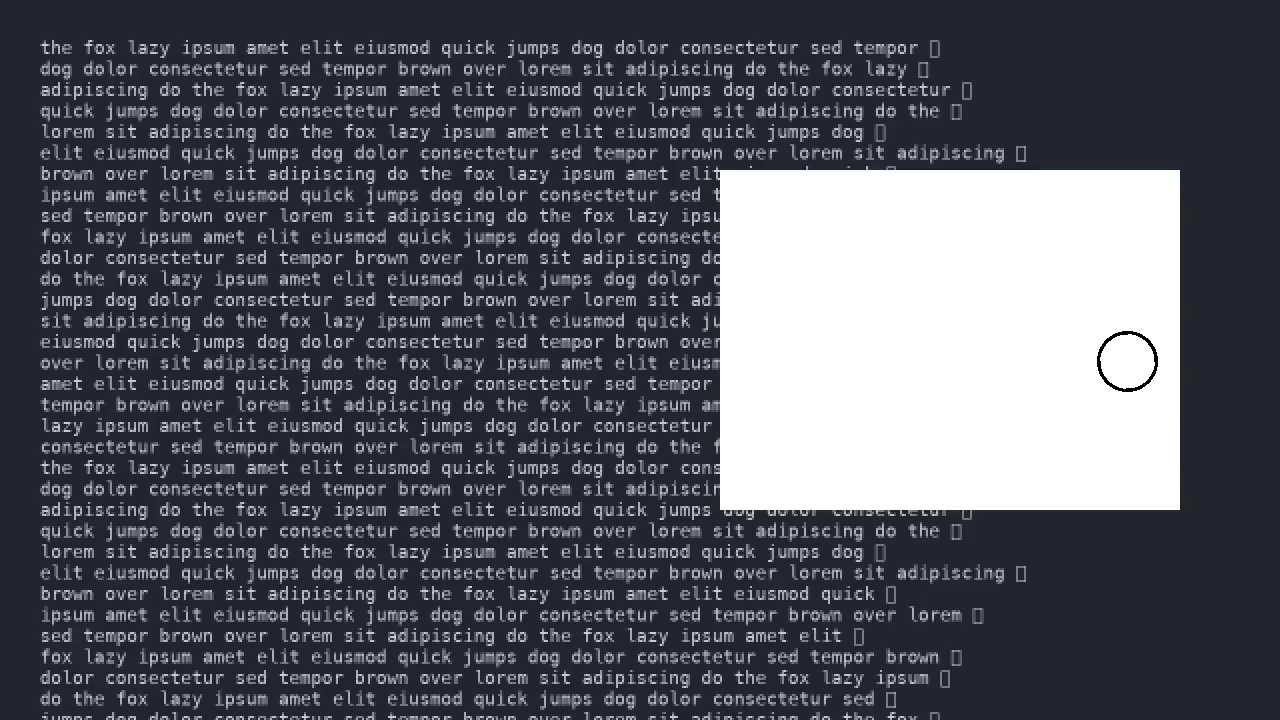
\includegraphics[width=\linewidth]{local-frame.png}\caption{Without a cover.}\end{subfigure}\hfill
  \begin{subfigure}{0.49\linewidth}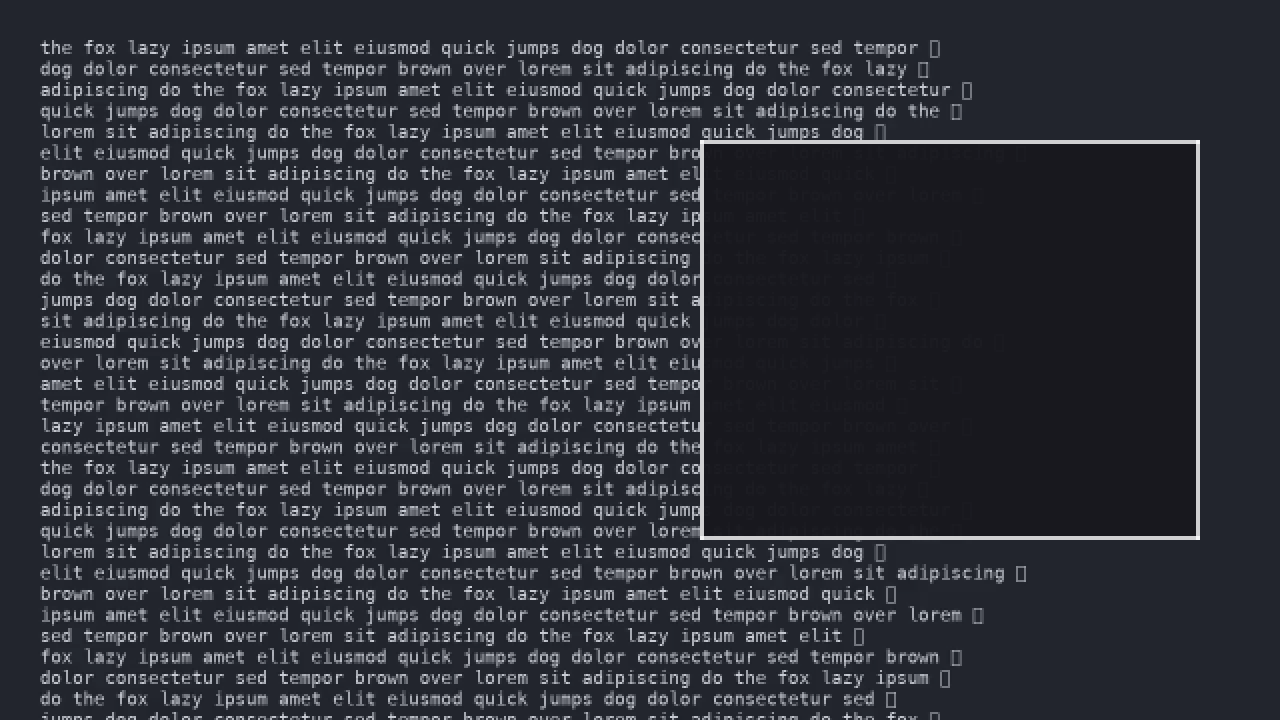
\includegraphics[width=\linewidth]{local-cover.png}\caption{The cover \guard{} computes at \SI{\LocalFirstCover}{\second}, drawn as it appears on screen.}\end{subfigure}
  \caption{The cover over the localised flash. It covers the flashing box with a one-cell margin, and the text beside it stays readable.}
  \label{fig:cover}
\end{figure}

% ---------------------------------------------------------------- 5
\section{Results}
\label{sec:results}

\subsection{Clips}

\Cref{tab:results} summarises five clips streamed through \guard{}'s pipeline exactly as captured frames arrive: decoded at 640 pixels wide, offered at their presentation times and resampled to 60 frames per second. Three fail: \psv{}'s colour example and two synthetic flashes, one localised and one full screen. Two pass and should never be covered: fast-scrolling text and \psv{}'s passing advertisement. Lead is how long before \psv{}'s first failing frame the first cover appeared.

\begin{table}[ht]
  \centering\small
  \caption{Clips streamed through \guard{} with the default settings. Times are from the start of each clip. A miss is a frame that \psv{} decided as failing that was not covered when shown.}
  \label{tab:results}
  \footnotesize\setlength{\tabcolsep}{4pt}
  \begin{tabular}{@{}lllrrrr@{}}
    \toprule
    Clip & Source & \psv{} verdict & First failing frame & First cover & Lead & Misses \\
    \midrule
    colors-epilepsy-warning & \psv{} example, \ColorsFPS{} fps & fails & \SI{\ColorsFirstFail}{\second} & \SI{\ColorsFirstCover}{\second} & \SI{0.15}{\second} & \ColorsMisses \\
    localised flash & synthetic, 60 fps & fails & \SI{\LocalFirstFail}{\second} & \SI{\LocalFirstCover}{\second} & \SI{0.30}{\second} & \LocalMisses \\
    full-screen flash & synthetic, 60 fps & fails & \SI{\FlashFirstFail}{\second} & \SI{\FlashFirstCover}{\second} & \SI{0.30}{\second} & \FlashMisses \\
    scrolling text & synthetic, 60 fps & passes & --- & never & --- & --- \\
    video-ad-sample-2 & \psv{} example, 23.98 fps & passes & --- & never & --- & --- \\
    \bottomrule
  \end{tabular}
\end{table}

\guard{}'s test suite runs the same pipeline on all four of \psv{}'s example videos and on synthetic clips of full-screen flashing, fast, slow and dark-mode scrolling text, and a sliding page. It fails if a failing clip is covered late or has misses, or if a passing clip is covered at all. On the remaining two failing examples, the first cover comes 0.23\,s and 2.8\,s before the first failing frame, with no misses.

\subsection{Live measurements}

On the development Mac, a laptop whose built-in Retina display of $1728\times1117$ points was analysed at $640\times414$:

\begin{itemize}
  \item Full-screen flashing played with \code{ffplay} was covered 323--352\,ms after it first appeared on screen, and 6--35\,ms after the frame that triggered the cover.
  \item A failing example filling about 30\% of a full-screen scene, beside \guard{}'s panel, was covered with no misses (\cref{fig:screens}).
  \item The cover falsely started by macOS's exit-from-full-screen animation was withdrawn in about 85\,ms, before its fade-in completed.
  \item With one display, \guard{} used 61--85\% of one CPU core, almost all of it in \code{Watch}, and 140--320\,MB of memory. \psv{}'s region search allocates several megabytes per frame while the screen flashes, so \guard{} sets a soft memory limit of 256\,MiB.
\end{itemize}

\begin{figure}[ht]
  \centering
  \begin{subfigure}{0.49\linewidth}
\includegraphics[width=\linewidth]{before.png}\caption{Without \guard{}: a scene with a flashing clip, playing full screen.}\end{subfigure}\hfill
  \begin{subfigure}{0.49\linewidth}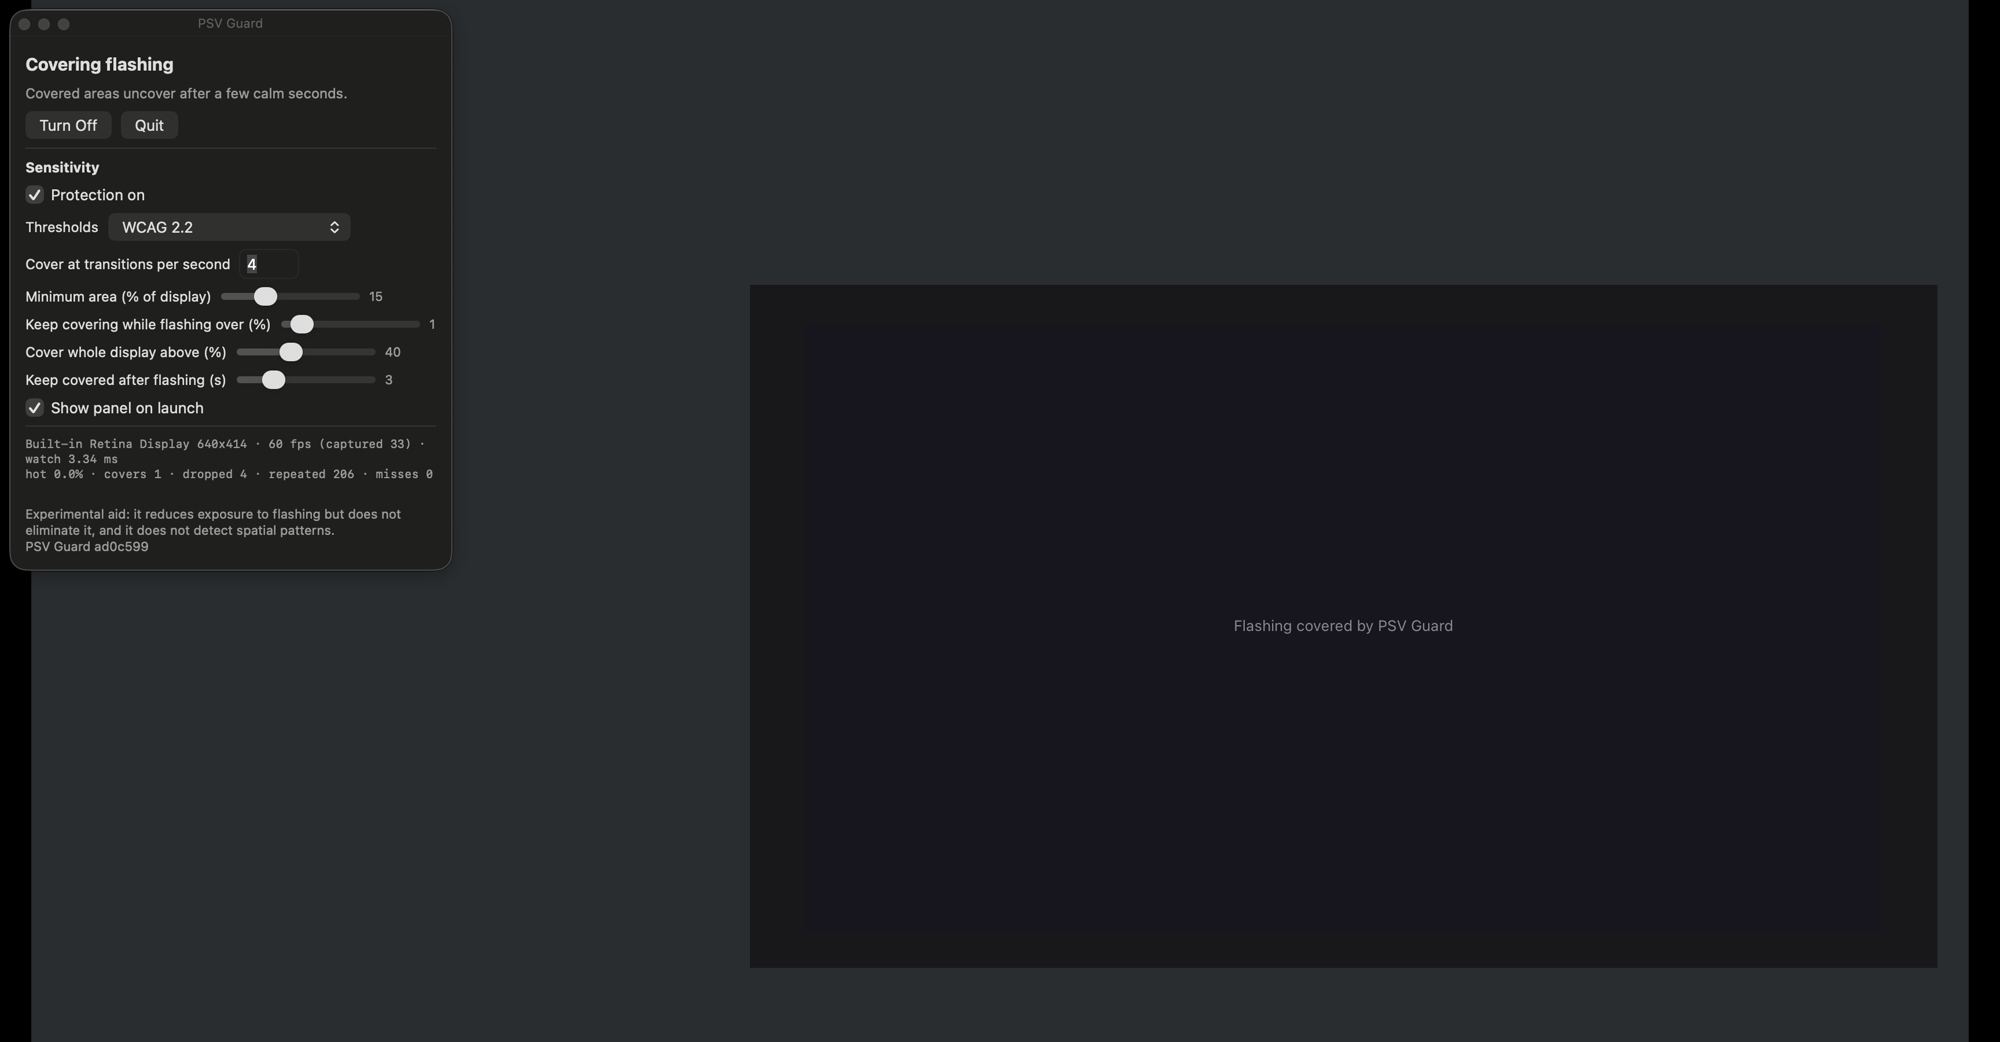
\includegraphics[width=\linewidth]{after.png}\caption{With \guard{}: the flashing area is covered, and the panel reports it.}\end{subfigure}\\[6pt]
  \begin{subfigure}{0.42\linewidth}\centering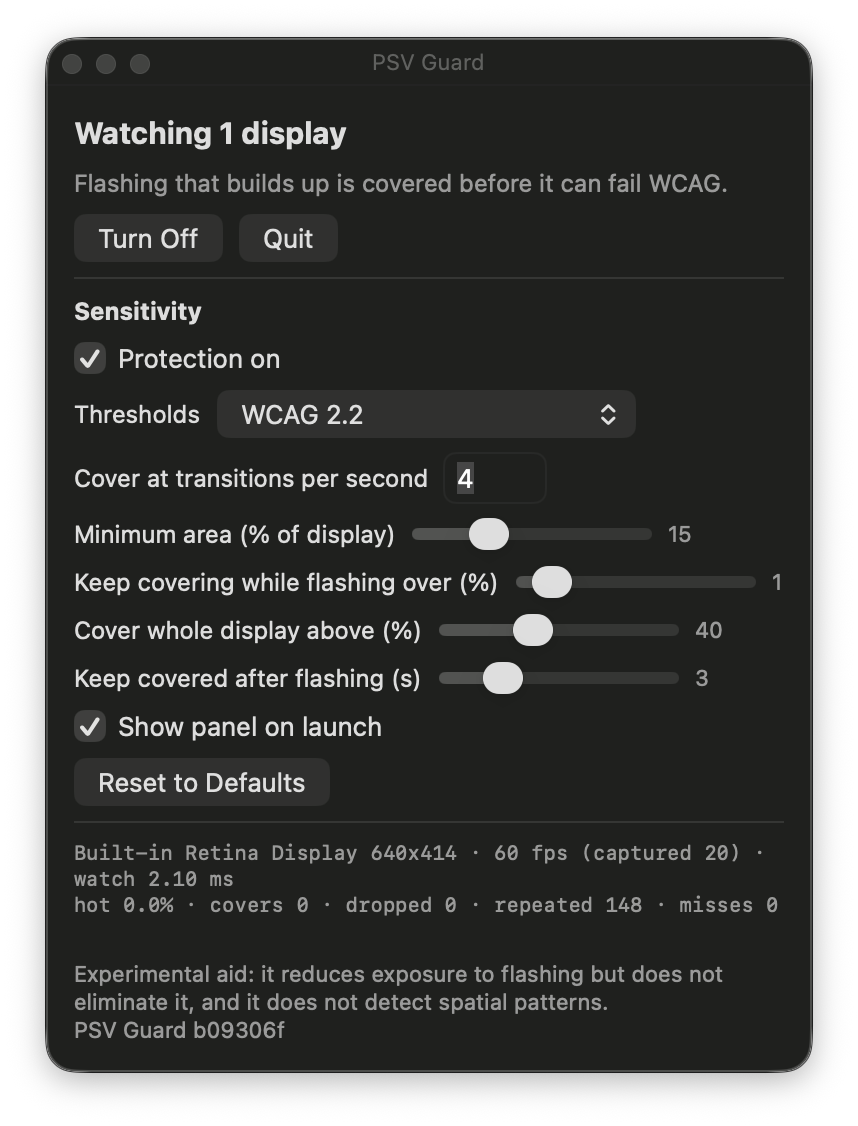
\includegraphics[width=0.78\linewidth]{panel.png}\caption{The panel: status, sensitivity settings, live statistics and the experimental-aid notice.}\end{subfigure}
  \caption{\guard{} running on macOS. Screen captures of the real app. The covers are normally excluded from all screen captures, so the cover shot used a build that allowed capturing them.}
  \label{fig:screens}
\end{figure}

% ---------------------------------------------------------------- 6
\section{Limits}
\label{sec:limits}

The measurements also show where \guard{} falls short. We report them as found.

\begin{description}[font=\bfseries\color{ink}]
  \item[Some flashing is always seen.] A cover needs evidence. With the defaults, the first cover follows the fourth transition, about a third of a second into full-screen flashing. The viewer sees those first flashes, which are below the guideline limit of three flashes but not harmless to everyone.
  \item[Small flashing waits for the backstop.] Flashing smaller than 15\% of the display, or flashing whose fill stays low from the start, is covered only by the backstop. That comes about a second after its first failing frame.
  \item[Unrelated motion can be covered.] Once one area starts a cover, every hot cell on the display is covered in that frame, including unrelated moving content. With a failing video and \psv{}'s passing advertisement playing side by side, the advertisement's moving logo was covered as well. Judging fill per region instead of per display would address this; it is a candidate change to the policy.
  \item[System animations hold covers back.] After a Space change, new covers wait 0.6\,s. A clip that flashed from its very first frame, as it entered full screen, showed 8 failing frames, about 0.13\,s, before it was covered.
  \item[The display is not modelled.] Luminance is relative, from 0 to 1. \psv{} does not model the display's absolute brightness, HDR or the viewer's distance. A very bright display makes the same content more intense than the thresholds assume.
  \item[Frame-exact concurrency.] A flash whose edge sweeps across a region over several frames is measured frame by frame, and may count as a smaller area than a viewer perceives.
  \item[Patterns are not detected.] Stripes, checkerboards and other regular patterns are a separate hazard in the guidelines, and neither \psv{} nor \guard{} checks them.
  \item[Cost.] Exact per-pixel analysis of every display at 60 frames per second costs most of a CPU core per display. Lower frame rates or capture widths trade cost against sensitivity.
  \item[Tuning data.] The default thresholds rest on four real videos and five synthetic clips. Other content may need tuning, and every threshold is a setting.
\end{description}

% ---------------------------------------------------------------- 7
\section{Conclusion}
\label{sec:conclusion}

The rules that protect broadcast viewers from flashing images can be applied to a computer screen as it is shown. \psv{} states the guidelines as exact rules on pixels: luminance and red transitions in linear light, merged ramps, alternation, a one-second count, and concurrent area found with summed-area tables. Its live mode separates what can be known at once, that a pixel flashes, from what takes a second, that nothing else does. \guard{} builds on that live measurement. A pixel count alone cannot separate flashing from moving detail. Combined with fill, a hold and a decided backstop, it covers flashing before its first failing frame on the clips measured here and leaves ordinary use uncovered.

The remaining work is clear from the limits. The policy should judge fill per region, so unrelated motion is never swept into a cover. It should reduce the hold-off after system animations, and it should cover small flashing sooner. Each change can be measured the same way: against \psv{}'s decided verdict, frame by frame. \guard{} cannot make an unchecked screen safe, but it can make that screen far less likely to show a full second of flashing.

% ---------------------------------------------------------------- Appendix
\appendix
\section{Default settings}
\label{app:settings}

\begin{table}[H]
  \centering\small
  \caption{\guard{}'s settings and defaults. Every setting is also a command-line flag.}
  \begin{tabularx}{\linewidth}{@{}llX@{}}
    \toprule
    Setting & Default & Effect \\
    \midrule
    \code{preset} & \code{wcag22} & \psv{} thresholds: \code{wcag22}, \code{trace24} or \code{broadcast} \\
    \code{hot-peak} & 4 & Transitions within a second at which a cell is hot \\
    \code{min-hot-area} & 15\% & Share of the display that must be hot before covering starts \\
    \code{flashing-area} & 1\% & Keep covers while this share of the display already flashes \\
    \code{full-area} & 40\% & Cover the whole display once this share is covered \\
    \code{calm} & 3\,s & Time a cell stays covered after it was last hot \\
    \code{fps} & 60 & Frames analysed per second per display \\
    \code{capture-width} & 640 & Width each display is scaled to for analysis \\
    \bottomrule
  \end{tabularx}
\end{table}

\section{Reproducing the figures}
\label{app:repro}

Every plot and mask image in this paper is generated from the clips by the program in \path{docs/whitepaper/figdata}. It drives \psv{}'s \code{Watch} and \guard{}'s monitor pipeline directly, then writes CSV data, images and the numbers quoted in the text. From the repository root:

\begin{verbatim}
go run -tags whitepaper ./docs/whitepaper/figdata
make -C docs/whitepaper
\end{verbatim}

The clip tests that guard the covering policy run with \code{make test}.

% ---------------------------------------------------------------- References
\begin{thebibliography}{99}\small
\bibitem{fisher2022} R.~S. Fisher et~al. Visually sensitive seizures: an updated review by the Epilepsy Foundation. \emph{Epilepsia}, 63(4):739--768, 2022. doi:10.1111/epi.17175.
\bibitem{harding2005} G.~Harding, A.~J. Wilkins, G.~Erba, G.~L. Barkley and R.~S. Fisher. Photic- and pattern-induced seizures: expert consensus of the Epilepsy Foundation of America Working Group. \emph{Epilepsia}, 46(9):1423--1425, 2005. doi:10.1111/j.1528-1167.2005.31305.x.
\bibitem{fisher2005review} R.~S. Fisher, G.~Harding, G.~Erba, G.~L. Barkley and A.~Wilkins. Photic- and pattern-induced seizures: a review for the Epilepsy Foundation of America Working Group. \emph{Epilepsia}, 46(9):1426--1441, 2005.
\bibitem{quirk1995} J.~A. Quirk, D.~R. Fish, S.~J.~M. Smith, J.~W.~A.~S. Sander, S.~D. Shorvon and P.~J. Allen. Incidence of photosensitive epilepsy: a prospective national study. \emph{Electroencephalography and Clinical Neurophysiology}, 95(4):260--267, 1995.
\bibitem{takahashi1998} T.~Takahashi and Y.~Tsukahara. Pocket Monster incident and low luminance visual stimuli: special reference to deep red flicker stimulation. \emph{Acta Paediatrica Japonica}, 40(6):631--637, 1998.
\bibitem{harding1994} G.~F.~A. Harding and P.~M. Jeavons. \emph{Photosensitive Epilepsy}. Mac Keith Press, London, 1994.
\bibitem{wcag22} World Wide Web Consortium. \emph{Web Content Accessibility Guidelines (WCAG) 2.2}, Success Criterion 2.3.1 Three Flashes or Below Threshold, and \emph{Understanding SC 2.3.1}. W3C Recommendation, 2023. \url{https://www.w3.org/TR/WCAG22/}.
\bibitem{itu1702} International Telecommunication Union. Recommendation ITU-R BT.1702: Guidance for the reduction of photosensitive epileptic seizures caused by television.
\bibitem{ofcom} Ofcom. Guidance Notes, Section Two: Harm and Offence (flashing images and regular patterns).
\bibitem{iso9241391} ISO 9241-391:2016. Ergonomics of human-system interaction --- Part 391: Requirements, analysis and compliance test methods for the reduction of photosensitive seizures.
\bibitem{tracemedia} Trace Research \& Development Center. PSE test media. \url{https://github.com/traceRERC/pse-test-media}.
\bibitem{srgb} IEC 61966-2-1:1999. Multimedia systems and equipment --- Colour measurement and management --- Part 2-1: Default RGB colour space --- sRGB.
\bibitem{cie015} CIE 015:2018. \emph{Colorimetry}, 4th edition. Commission Internationale de l'Éclairage, 2018.
\bibitem{crow1984} F.~C. Crow. Summed-area tables for texture mapping. \emph{Computer Graphics (Proceedings of SIGGRAPH)}, 18(3):207--212, 1984.
\bibitem{psv} B.~Nunez. psv: photosensitivity flash detection, version 0.2.0. \url{https://github.com/brian-nunez/psv}.
\bibitem{psvguard} B.~Nunez. PSV Guard. \url{https://github.com/brian-nunez/psvguard}.
\end{thebibliography}

\end{document}
